% ----------------------------------------------------------------------
%
%                            TFMTesis.tex
%
%----------------------------------------------------------------------
%
% Este fichero contiene el "documento maestro" del documento. Lo único
% que hace es configurar el entorno LaTeX e incluir los ficheros .tex
% que contienen cada sección.
%
%----------------------------------------------------------------------
%
% Los ficheros necesarios para este documento son:
%
%       TeXiS/* : ficheros de la plantilla TeXiS.
%       Cascaras/* : ficheros con las partes del documento que no
%          son capítulos ni apéndices (portada, agradecimientos, etc.)
%       Capitulos/*.tex : capítulos de la tesis
%       Apendices/*.tex: apéndices de la tesis
%       constantes.tex: constantes LaTeX
%       config.tex : configuración de la "compilación" del documento
%       guionado.tex : palabras con guiones
%
% Para la bibliografía, además, se necesitan:
%
%       *.bib : ficheros con la información de las referencias
%
% ---------------------------------------------------------------------

\documentclass[11pt,a4paper,twoside]{book}

%
% Definimos  el   comando  \compilaCapitulo,  que   luego  se  utiliza
% (opcionalmente) en config.tex. Quedaría  mejor si también se definiera
% en  ese fichero,  pero por  el modo  en el  que funciona  eso  no es
% posible. Puedes consultar la documentación de ese fichero para tener
% más  información. Definimos también  \compilaApendice, que  tiene el
% mismo  cometido, pero  que se  utiliza para  compilar  únicamente un
% apéndice.
%
%
% Si  queremos   compilar  solo   una  parte  del   documento  podemos
% especificar mediante  \includeonly{...} qué ficheros  son los únicos
% que queremos  que se incluyan.  Esto  es útil por  ejemplo para sólo
% compilar un capítulo.
%
% El problema es que todos aquellos  ficheros que NO estén en la lista
% NO   se  incluirán...  y   eso  también   afecta  a   ficheros  de
% la plantilla...
%
% Total,  que definimos  una constante  con los  ficheros  que siempre
% vamos a querer compilar  (aquellos relacionados con configuración) y
% luego definimos \compilaCapitulo.
\newcommand{\ficherosBasicosTeXiS}{%
TeXiS/TeXiS_pream,TeXiS/TeXiS_cab,TeXiS/TeXiS_bib,TeXiS/TeXiS_cover%
}
\newcommand{\ficherosBasicosTexto}{%
constantes,guionado,Cascaras/bibliografia,config%
}
\newcommand{\compilaCapitulo}[1]{%
\includeonly{\ficherosBasicosTeXiS,\ficherosBasicosTexto,Capitulos/#1}%
}

\newcommand{\compilaApendice}[1]{%
\includeonly{\ficherosBasicosTeXiS,\ficherosBasicosTexto,Apendices/#1}%
}

%- - - - - - - - - - - - - - - - - - - - - - - - - - - - - - - - - - -
%            Preámbulo del documento. Configuraciones varias
%- - - - - - - - - - - - - - - - - - - - - - - - - - - - - - - - - - -

% Define  el  tipo  de  compilación que  estamos  haciendo.   Contiene
% definiciones  de  constantes que  cambian  el  comportamiento de  la
% compilación. Debe incluirse antes del paquete TeXiS/TeXiS.sty
%---------------------------------------------------------------------
%
%                          config.tex
%
%---------------------------------------------------------------------
%
% Contiene la  definición de constantes  que determinan el modo  en el
% que se compilará el documento.
%
%---------------------------------------------------------------------
%
% En concreto, podemos  indicar si queremos "modo release",  en el que
% no  aparecerán  los  comentarios  (creados  mediante  \com{Texto}  o
% \comp{Texto}) ni los "por  hacer" (creados mediante \todo{Texto}), y
% sí aparecerán los índices. El modo "debug" (o mejor dicho en modo no
% "release" muestra los índices  (construirlos lleva tiempo y son poco
% útiles  salvo  para   la  versión  final),  pero  sí   el  resto  de
% anotaciones.
%
% Si se compila con LaTeX (no  con pdflatex) en modo Debug, también se
% muestran en una esquina de cada página las entradas (en el índice de
% palabras) que referencian  a dicha página (consulta TeXiS_pream.tex,
% en la parte referente a show).
%
% El soporte para  el índice de palabras en  TeXiS es embrionario, por
% lo  que no  asumas que  esto funcionará  correctamente.  Consulta la
% documentación al respecto en TeXiS_pream.tex.
%
%
% También  aquí configuramos  si queremos  o  no que  se incluyan  los
% acrónimos  en el  documento final  en la  versión release.  Para eso
% define (o no) la constante \acronimosEnRelease.
%
% Utilizando \compilaCapitulo{nombre}  podemos también especificar qué
% capítulo(s) queremos que se compilen. Si no se pone nada, se compila
% el documento  completo.  Si se pone, por  ejemplo, 01Introduccion se
% compilará únicamente el fichero Capitulos/01Introduccion.tex
%
% Para compilar varios  capítulos, se separan sus nombres  con comas y
% no se ponen espacios de separación.
%
% En realidad  la macro \compilaCapitulo  está definida en  el fichero
% principal tesis.tex.
%
%---------------------------------------------------------------------


% Comentar la línea si no se compila en modo release.
% TeXiS hará el resto.
% ¡¡¡Si cambias esto, haz un make clean antes de recompilar!!!
\def\release{1}


% Descomentar la linea si se quieren incluir los
% acrónimos en modo release (en modo debug
% no se incluirán nunca).
% ¡¡¡Si cambias esto, haz un make clean antes de recompilar!!!
%\def\acronimosEnRelease{1}


% Descomentar la línea para establecer el capítulo que queremos
% compilar

% \compilaCapitulo{01Introduccion}
% \compilaCapitulo{02EstructuraYGeneracion}
% \compilaCapitulo{03Edicion}
% \compilaCapitulo{04Imagenes}
% \compilaCapitulo{05Bibliografia}
% \compilaCapitulo{06Makefile}

% \compilaApendice{01AsiSeHizo}

% Variable local para emacs, para  que encuentre el fichero maestro de
% compilación y funcionen mejor algunas teclas rápidas de AucTeX
%%%
%%% Local Variables:
%%% mode: latex
%%% TeX-master: "./Tesis.tex"
%%% End:


% Paquete de la plantilla
\usepackage{TeXiS/TeXiS}

% Incluimos el fichero con comandos de constantes
%---------------------------------------------------------------------
%
%                          constantes.tex
%
%---------------------------------------------------------------------
%
% Fichero que  declara nuevos comandos LaTeX  sencillos realizados por
% comodidad en la escritura de determinadas palabras
%
%---------------------------------------------------------------------

%%%%%%%%%%%%%%%%%%%%%%%%%%%%%%%%%%%%%%%%%%%%%%%%%%%%%%%%%%%%%%%%%%%%%%
% Comando: 
%
%       \titulo
%
% Resultado: 
%
% Escribe el título del documento.
%%%%%%%%%%%%%%%%%%%%%%%%%%%%%%%%%%%%%%%%%%%%%%%%%%%%%%%%%%%%%%%%%%%%%%
\def\titulo{\textsc{TeXiS}: Una plantilla de \LaTeX\
  para Tesis y otros documentos}

%%%%%%%%%%%%%%%%%%%%%%%%%%%%%%%%%%%%%%%%%%%%%%%%%%%%%%%%%%%%%%%%%%%%%%
% Comando: 
%
%       \autor
%
% Resultado: 
%
% Escribe el autor del documento.
%%%%%%%%%%%%%%%%%%%%%%%%%%%%%%%%%%%%%%%%%%%%%%%%%%%%%%%%%%%%%%%%%%%%%%
\def\autor{Marco Antonio y Pedro Pablo G\'omez Mart\'in}

% Variable local para emacs, para  que encuentre el fichero maestro de
% compilación y funcionen mejor algunas teclas rápidas de AucTeX

%%%
%%% Local Variables:
%%% mode: latex
%%% TeX-master: "tesis.tex"
%%% End:


% Sacamos en el log de la compilación el copyright
%\typeout{Copyright Marco Antonio and Pedro Pablo Gomez Martin}

%
% "Metadatos" para el PDF
%
\ifpdf\hypersetup{%
    pdftitle = {\titulo},
    pdfsubject = {Plantilla de Tesis},
    pdfkeywords = {Plantilla, LaTeX, tesis, trabajo de
      investigación, trabajo de Master},
    pdfauthor = {\textcopyright\ \autor},
    pdfcreator = {\LaTeX\ con el paquete \flqq hyperref\frqq},
    pdfproducer = {pdfeTeX-0.\the\pdftexversion\pdftexrevision},
    }
    \pdfinfo{/CreationDate (\today)}
\fi


%- - - - - - - - - - - - - - - - - - - - - - - - - - - - - - - - - - -
%                        Documento
%- - - - - - - - - - - - - - - - - - - - - - - - - - - - - - - - - - -
\begin{document}

% Incluimos el  fichero de definición de guionado  de algunas palabras
% que LaTeX no ha dividido como debería
%----------------------------------------------------------------
%
%                          guionado.tex
%
%----------------------------------------------------------------
%
% Fichero con algunas divisiones de palabras que LaTeX no
% hace correctamente si no se le da alguna ayuda.
%
%----------------------------------------------------------------

\hyphenation{
% a
abs-trac-to
abs-trac-tos
abs-trac-ta
abs-trac-tas
ac-tua-do-res
a-gra-de-ci-mien-tos
ana-li-za-dor
an-te-rio-res
an-te-rior-men-te
apa-rien-cia
a-pro-pia-do
a-pro-pia-dos
a-pro-pia-da
a-pro-pia-das
a-pro-ve-cha-mien-to
a-que-llo
a-que-llos
a-que-lla
a-que-llas
a-sig-na-tu-ra
a-sig-na-tu-ras
a-so-cia-da
a-so-cia-das
a-so-cia-do
a-so-cia-dos
au-to-ma-ti-za-do
% b
batch
bi-blio-gra-fía
bi-blio-grá-fi-cas
bien
bo-rra-dor
boo-l-ean-expr
% c
ca-be-ce-ra
call-me-thod-ins-truc-tion
cas-te-lla-no
cir-cuns-tan-cia
cir-cuns-tan-cias
co-he-ren-te
co-he-ren-tes
co-he-ren-cia
co-li-bri
co-men-ta-rio
co-mer-cia-les
co-no-ci-mien-to
cons-cien-te
con-si-de-ra-ba
con-si-de-ra-mos
con-si-de-rar-se
cons-tan-te
cons-trucción
cons-tru-ye
cons-tru-ir-se
con-tro-le
co-rrec-ta-men-te
co-rres-pon-den
co-rres-pon-dien-te
co-rres-pon-dien-tes
co-ti-dia-na
co-ti-dia-no
crean
cris-ta-li-zan
cu-rri-cu-la
cu-rri-cu-lum
cu-rri-cu-lar
cu-rri-cu-la-res
% d
de-di-ca-do
de-di-ca-dos
de-di-ca-da
de-di-ca-das
de-rro-te-ro
de-rro-te-ros
de-sa-rro-llo
de-sa-rro-llos
de-sa-rro-lla-do
de-sa-rro-lla-dos
de-sa-rro-lla-da
de-sa-rro-lla-das
de-sa-rro-lla-dor
de-sa-rro-llar
des-cri-bi-re-mos
des-crip-ción
des-crip-cio-nes
des-cri-to
des-pués
de-ta-lla-do
de-ta-lla-dos
de-ta-lla-da
de-ta-lla-das
di-a-gra-ma
di-a-gra-mas
di-se-ños
dis-po-ner
dis-po-ni-bi-li-dad
do-cu-men-ta-da
do-cu-men-to
do-cu-men-tos
% e
edi-ta-do
e-du-ca-ti-vo
e-du-ca-ti-vos
e-du-ca-ti-va
e-du-ca-ti-vas
e-la-bo-ra-do
e-la-bo-ra-dos
e-la-bo-ra-da
e-la-bo-ra-das
es-co-llo
es-co-llos
es-tu-dia-do
es-tu-dia-dos
es-tu-dia-da
es-tu-dia-das
es-tu-dian-te
e-va-lua-cio-nes
e-va-lua-do-res
exis-ten-tes
exhaus-ti-va
ex-pe-rien-cia
ex-pe-rien-cias
% f
for-ma-li-za-do
% g
ge-ne-ra-ción
ge-ne-ra-dor
ge-ne-ra-do-res
ge-ne-ran
% h
he-rra-mien-ta
he-rra-mien-tas
% i
i-dio-ma
i-dio-mas
im-pres-cin-di-ble
im-pres-cin-di-bles
in-de-xa-do
in-de-xa-dos
in-de-xa-da
in-de-xa-das
in-di-vi-dual
in-fe-ren-cia
in-fe-ren-cias
in-for-ma-ti-ca
in-gre-dien-te
in-gre-dien-tes
in-me-dia-ta-men-te
ins-ta-la-do
ins-tan-cias
% j
% k
% l
len-gua-je
li-be-ra-to-rio
li-be-ra-to-rios
li-be-ra-to-ria
li-be-ra-to-rias
li-mi-ta-do
li-te-ra-rio
li-te-ra-rios
li-te-ra-ria
li-te-ra-rias
lo-tes
% m
ma-ne-ra
ma-nual
mas-que-ra-de
ma-yor
me-mo-ria
mi-nis-te-rio
mi-nis-te-rios
mo-de-lo
mo-de-los
mo-de-la-do
mo-du-la-ri-dad
mo-vi-mien-to
% n
na-tu-ral
ni-vel
nues-tro
% o
obs-tan-te
o-rien-ta-do
o-rien-ta-dos
o-rien-ta-da
o-rien-ta-das
% p
pa-ra-le-lo
pa-ra-le-la
par-ti-cu-lar
par-ti-cu-lar-men-te
pe-da-gó-gi-ca
pe-da-gó-gi-cas
pe-da-gó-gi-co
pe-da-gó-gi-cos
pe-rio-di-ci-dad
per-so-na-je
plan-te-a-mien-to
plan-te-a-mien-tos
po-si-ción
pre-fe-ren-cia
pre-fe-ren-cias
pres-cin-di-ble
pres-cin-di-bles
pri-me-ra
pro-ble-ma
pro-ble-mas
pró-xi-mo
pu-bli-ca-cio-nes
pu-bli-ca-do
% q
% r
rá-pi-da
rá-pi-do
ra-zo-na-mien-to
ra-zo-na-mien-tos
re-a-li-zan-do
re-fe-ren-cia
re-fe-ren-cias
re-fe-ren-cia-da
re-fe-ren-cian
re-le-van-tes
re-pre-sen-ta-do
re-pre-sen-ta-dos
re-pre-sen-ta-da
re-pre-sen-ta-das
re-pre-sen-tar-lo
re-qui-si-to
re-qui-si-tos
res-pon-der
res-pon-sa-ble
% s
se-pa-ra-do
si-guien-do
si-guien-te
si-guien-tes
si-guie-ron
si-mi-lar
si-mi-la-res
si-tua-ción
% t
tem-pe-ra-ments
te-ner
trans-fe-ren-cia
trans-fe-ren-cias
% u
u-sua-rio
Unreal-Ed
% v
va-lor
va-lo-res
va-rian-te
ver-da-de-ro
ver-da-de-ros
ver-da-de-ra
ver-da-de-ras
ver-da-de-ra-men-te
ve-ri-fi-ca
% w
% x
% y
% z
}
% Variable local para emacs, para que encuentre el fichero
% maestro de compilación
%%%
%%% Local Variables:
%%% mode: latex
%%% TeX-master: "./Tesis.tex"
%%% End:


% Marcamos  el inicio  del  documento para  la  numeración de  páginas
% (usando números romanos para esta primera fase).
\frontmatter
\pagestyle{empty}

%---------------------------------------------------------------------
%
%                          configCover.tex
%
%---------------------------------------------------------------------
%
% cover.tex
% Copyright 2009 Marco Antonio Gomez-Martin, Pedro Pablo Gomez-Martin
%
% This file belongs to the TeXiS manual, a LaTeX template for writting
% Thesis and other documents. The complete last TeXiS package can
% be obtained from http://gaia.fdi.ucm.es/projects/texis/
%
% Although the TeXiS template itself is distributed under the 
% conditions of the LaTeX Project Public License
% (http://www.latex-project.org/lppl.txt), the manual content
% uses the CC-BY-SA license that stays that you are free:
%
%    - to share & to copy, distribute and transmit the work
%    - to remix and to adapt the work
%
% under the following conditions:
%
%    - Attribution: you must attribute the work in the manner
%      specified by the author or licensor (but not in any way that
%      suggests that they endorse you or your use of the work).
%    - Share Alike: if you alter, transform, or build upon this
%      work, you may distribute the resulting work only under the
%      same, similar or a compatible license.
%
% The complete license is available in
% http://creativecommons.org/licenses/by-sa/3.0/legalcode
%
%---------------------------------------------------------------------
%
% Fichero que contiene la configuración de la portada y de la 
% primera hoja del documento.
%
%---------------------------------------------------------------------


% Pueden configurarse todos los elementos del contenido de la portada
% utilizando comandos.

%%%%%%%%%%%%%%%%%%%%%%%%%%%%%%%%%%%%%%%%%%%%%%%%%%%%%%%%%%%%%%%%%%%%%%
% Título del documento:
% \tituloPortada{titulo}
% Nota:
% Si no se define se utiliza el del \titulo. Este comando permite
% cambiar el título de forma que se especifiquen dónde se quieren
% los retornos de carro cuando se utilizan fuentes grandes.
%%%%%%%%%%%%%%%%%%%%%%%%%%%%%%%%%%%%%%%%%%%%%%%%%%%%%%%%%%%%%%%%%%%%%%
\tituloPortada{
%Título en español \textcolor{red}{(definido en Cascaras$\backslash$cover.tex)}
Explicaciones para un recomendador de música basadas en datos enlazados
}


%%%%%%%%%%%%%%%%%%%%%%%%%%%%%%%%%%%%%%%%%%%%%%%%%%%%%%%%%%%%%%%%%%%%%%
% Título del documento en inglés:
% \tituloPortadaEng{titulo}
% Nota:
% Si no se define se utiliza el del \titulo. Este comando permite
% cambiar el título de forma que se especifiquen dónde se quieren
% los retornos de carro cuando se utilizan fuentes grandes.
%%%%%%%%%%%%%%%%%%%%%%%%%%%%%%%%%%%%%%%%%%%%%%%%%%%%%%%%%%%%%%%%%%%%%%
\tituloPortadaEng{%
Title in English \textcolor{red}{(defined in Cascaras$\backslash$cover.tex)}
}

%%%%%%%%%%%%%%%%%%%%%%%%%%%%%%%%%%%%%%%%%%%%%%%%%%%%%%%%%%%%%%%%%%%%%%
% Autor del documento:
% \autorPortada{Nombre}
% Se utiliza en la portada y en el valor por defecto del
% primer subtítulo de la segunda portada.
%%%%%%%%%%%%%%%%%%%%%%%%%%%%%%%%%%%%%%%%%%%%%%%%%%%%%%%%%%%%%%%%%%%%%%
\autorPortada{%\textcolor{red}{Nombre Apellido1 Apellido2}
Adrián Garrido Sierra\\Diego Sánchez Muniesa}

%%%%%%%%%%%%%%%%%%%%%%%%%%%%%%%%%%%%%%%%%%%%%%%%%%%%%%%%%%%%%%%%%%%%%%
% Fecha de publicación:
% \fechaPublicacion{Fecha}
% Puede ser vacío. Aparece en la última línea de ambas portadas
%%%%%%%%%%%%%%%%%%%%%%%%%%%%%%%%%%%%%%%%%%%%%%%%%%%%%%%%%%%%%%%%%%%%%%
% Descomentar para que ponga siempre la fecha actual
%\fechaPublicacion{\today}
\fechaPublicacion{\textcolor{red}{DIA de MES de AÑO}}

%%%%%%%%%%%%%%%%%%%%%%%%%%%%%%%%%%%%%%%%%%%%%%%%%%%%%%%%%%%%%%%%%%%%%%
% Imagen de la portada (y escala)
% \imagenPortada{Fichero}
% \escalaImagenPortada{Numero}
% Si no se especifica, se utiliza la imagen TODO.pdf
%%%%%%%%%%%%%%%%%%%%%%%%%%%%%%%%%%%%%%%%%%%%%%%%%%%%%%%%%%%%%%%%%%%%%%
% imagen en blanco y negro
%\imagenPortada{Imagenes/Vectorial/escudoUCM}
%imagen en color
\imagenPortada{Imagenes/Bitmap/escudoUCMcolor}
\escalaImagenPortada{.2}

%%%%%%%%%%%%%%%%%%%%%%%%%%%%%%%%%%%%%%%%%%%%%%%%%%%%%%%%%%%%%%%%%%%%%%
% Tipo de documento.
% \tipoDocumento{Tipo}
% Para el texto justo debajo del escudo.
% Si no se indica, se utiliza "TESIS DOCTORAL".
%%%%%%%%%%%%%%%%%%%%%%%%%%%%%%%%%%%%%%%%%%%%%%%%%%%%%%%%%%%%%%%%%%%%%%
\tipoDocumento{Trabajo de Fin de Grado}

%%%%%%%%%%%%%%%%%%%%%%%%%%%%%%%%%%%%%%%%%%%%%%%%%%%%%%%%%%%%%%%%%%%%%%
% Institución/departamento asociado al documento.
% \institucion{Nombre}
% Puede tener varias líneas. Se utiliza en las dos portadas.
% Si no se indica aparecerá vacío.
%%%%%%%%%%%%%%%%%%%%%%%%%%%%%%%%%%%%%%%%%%%%%%%%%%%%%%%%%%%%%%%%%%%%%%
\institucion{%
Grado en \textcolor{red}{Ingeniería Informática}\\[0.2em]
Facultad de Informática\\[0.2em]
Universidad Complutense de Madrid
}

%%%%%%%%%%%%%%%%%%%%%%%%%%%%%%%%%%%%%%%%%%%%%%%%%%%%%%%%%%%%%%%%%%%%%%
% Director del trabajo.
% \directorPortada{Nombre}
% Se utiliza para el valor por defecto del segundo subtítulo, donde
% se indica quién es el director del trabajo.
% Si se fuerza un subtítulo distinto, no hace falta definirlo.
%%%%%%%%%%%%%%%%%%%%%%%%%%%%%%%%%%%%%%%%%%%%%%%%%%%%%%%%%%%%%%%%%%%%%%
\directorPortada{%\textcolor{red}{Director 1\\Director 2}
Guillermo Jiménez Díaz\\Marta Caro Martínez}


%%%%%%%%%%%%%%%%%%%%%%%%%%%%%%%%%%%%%%%%%%%%%%%%%%%%%%%%%%%%%%%%%%%%%%
% Colaborador en la dirección del trabajo.
% \colaboradorPortada{Nombre}
% Se utiliza para el valor por defecto del segundo subtítulo, donde
% se indica quién es el colaborador en la dirección del trabajo.
% Si se fuerza un subtítulo distinto, no hace falta definirlo.
%%%%%%%%%%%%%%%%%%%%%%%%%%%%%%%%%%%%%%%%%%%%%%%%%%%%%%%%%%%%%%%%%%%%%%
\colaboradorPortada{\textcolor{red}{Colaborador 1\\Colaborador 2}}


%%%%%%%%%%%%%%%%%%%%%%%%%%%%%%%%%%%%%%%%%%%%%%%%%%%%%%%%%%%%%%%%%%%%%%
% Texto del primer subtítulo de la segunda portada.
% \textoPrimerSubtituloPortada{Texto}
% Para configurar el primer "texto libre" de la segunda portada.
% Si no se especifica se indica "Memoria que presenta para optar al
% título de Doctor en Informática" seguido del \autorPortada.
%%%%%%%%%%%%%%%%%%%%%%%%%%%%%%%%%%%%%%%%%%%%%%%%%%%%%%%%%%%%%%%%%%%%%%
\textoPrimerSubtituloPortada{%
\textbf{Trabajo de Fin de Grado en \textcolor{red}{Ingeniería Informática}}  \\ [0.3em]
\textbf{Departamento de \textcolor{red}{XXXXXXXXXXXXX}} \\ [0.3em]
}

%%%%%%%%%%%%%%%%%%%%%%%%%%%%%%%%%%%%%%%%%%%%%%%%%%%%%%%%%%%%%%%%%%%%%%
% Texto del segundo subtítulo de la segunda portada.
% \textoSegundoSubtituloPortada{Texto}
% Para configurar el segundo "texto libre" de la segunda portada.
% Si no se especifica se indica "Dirigida por el Doctor" seguido
% del \directorPortada.
%%%%%%%%%%%%%%%%%%%%%%%%%%%%%%%%%%%%%%%%%%%%%%%%%%%%%%%%%%%%%%%%%%%%%%
\textoSegundoSubtituloPortada{%
\textbf{Convocatoria: }\textit{\textcolor{red}{Febrero/Junio/Septiembre} \the\year} \\ [0.2em]
\textbf{Calificación: }\textit{\textcolor{red}{Nota}}
}

%%%%%%%%%%%%%%%%%%%%%%%%%%%%%%%%%%%%%%%%%%%%%%%%%%%%%%%%%%%%%%%%%%%%%%
% \explicacionDobleCara
% Si se utiliza, se aclara que el documento está preparado para la
% impresión a doble cara.
%%%%%%%%%%%%%%%%%%%%%%%%%%%%%%%%%%%%%%%%%%%%%%%%%%%%%%%%%%%%%%%%%%%%%%
%\explicacionDobleCara

%%%%%%%%%%%%%%%%%%%%%%%%%%%%%%%%%%%%%%%%%%%%%%%%%%%%%%%%%%%%%%%%%%%%%%
% \isbn
% Si se utiliza, aparecerá el ISBN detrás de la segunda portada.
%%%%%%%%%%%%%%%%%%%%%%%%%%%%%%%%%%%%%%%%%%%%%%%%%%%%%%%%%%%%%%%%%%%%%%
%\isbn{978-84-692-7109-4}


%%%%%%%%%%%%%%%%%%%%%%%%%%%%%%%%%%%%%%%%%%%%%%%%%%%%%%%%%%%%%%%%%%%%%%
% \copyrightInfo
% Si se utiliza, aparecerá información de los derechos de copyright
% detrás de la segunda portada.
%%%%%%%%%%%%%%%%%%%%%%%%%%%%%%%%%%%%%%%%%%%%%%%%%%%%%%%%%%%%%%%%%%%%%%
%\copyrightInfo{\autor}


%%
%% Creamos las portadas
%%
\makeCover

% Variable local para emacs, para que encuentre el fichero
% maestro de compilación
%%%
%%% Local Variables:
%%% mode: latex
%%% TeX-master: "../Tesis.tex"
%%% End:

%\chapter*{Autorización de difusión}

   
El abajo firmante, matriculado en el Máster en Ingeniería en Informática de la Facultad de Informática, autoriza a la Universidad Complutense de Madrid (UCM) a difundir y utilizar con fines académicos, no comerciales y mencionando expresamente a su autor el presente Trabajo Fin de Máster: ``TITULO DEL TRABAJO'', realizado durante el curso académico CURSO bajo la dirección de DIRECTORES en el Departamento de XXXXXXXXXXXXXXXXXXXXXXXX, y a la Biblioteca de la UCM a depositarlo en el Archivo Institucional E-Prints Complutense con el objeto de incrementar la difusión, uso e impacto del trabajo en Internet y garantizar su preservación y acceso a largo plazo.

\vspace{5cm}

% +--------------------------------------------------------------------+
% | On the line below, replace "Enter Your Name" with your name
% | Use the same form of your name as it appears on your title page.
% | Use mixed case, for example, Lori Goetsch.
% +--------------------------------------------------------------------+
\begin{center}
	\large Nombre Del Alumno\\
	
	\vspace{0.5cm}
	
	% +--------------------------------------------------------------------+
	% | On the line below, replace Fecha
	% |
	% +--------------------------------------------------------------------+
	
	\today\\
	
\end{center}

%% +--------------------------------------------------------------------+
% | Dedication Page (Optional)
% +--------------------------------------------------------------------+

\chapter*{Dedicatoria}

\begin{flushright}
\begin{minipage}[c]{8.5cm}
\flushright{\textit{A Pedro Pablo y Marco Antonio, por crear TeXiS e iluminar nuestro camino}}
\end{minipage}
\end{flushright}
%% +--------------------------------------------------------------------+
% | Acknowledgements Page (Optional)                                   |
% +--------------------------------------------------------------------+

\chapter*{Agradecimientos}

A Guillermo, por el tiempo empleado en hacer estas plantillas. A Adrián, Enrique y Nacho, por sus comentarios para mejorar lo que hicimos. Y a Narciso, a quien no le ha hecho falta el Anillo Único para coordinarnos a todos.












\chapter*{Resumen}

\section*{\tituloPortadaVal}

Los sistemas de recomendación proporcionan a los usuarios opciones seleccionadas en base a sus preferencias, aportándoles una forma cómoda y rápida de encontrar elementos de interés. Para que este proceso sea efectivo, sin embargo, el usuario debe comprender las recomendaciones y confiar en el sistema para encontrar lo que busca. Esta confianza puede lograrse mediante el uso de explicaciones, que son una forma intuitiva de justificar la elección de las recomendaciones de forma comprensible para el usuario.\\

Este trabajo busca enriquecer las explicaciones para un recomendador de música gracias a los datos enlazados. Se hará un estudio de esta tecnología y las formas en que puede aplicarse al ámbito de los sistemas de recomendación y se demostrará de forma práctica con el desarrollo del prototipo de una aplicación que obtenga y muestre explicaciones para el recomendador mencionado.\\


\section*{Palabras clave}
   
\noindent Datos enlazados, web semántica, explicaciones, RDF, SPARQL.

   



\begin{otherlanguage}{english}
\chapter*{Abstract}

\section*{\tituloPortadaEngVal}

An abstract in English, half a page long, including the title in English. Below, a list with no more than 10 keywords.


\section*{Keywords}

\noindent Linked Data, semantic web, explanations, RDF, SPARQL.




% Si el trabajo se escribe en inglés, comentar esta línea y descomentar
% otra igual que hay justo antes de \end{document}
\end{otherlanguage}

\ifx\generatoc\undefined
\else
%---------------------------------------------------------------------
%
%                          TeXiS_toc.tex
%
%---------------------------------------------------------------------
%
% TeXiS_toc.tex
% Copyright 2009 Marco Antonio Gomez-Martin, Pedro Pablo Gomez-Martin
%
% This file belongs to TeXiS, a LaTeX template for writting
% Thesis and other documents. The complete last TeXiS package can
% be obtained from http://gaia.fdi.ucm.es/projects/texis/
%
% This work may be distributed and/or modified under the
% conditions of the LaTeX Project Public License, either version 1.3
% of this license or (at your option) any later version.
% The latest version of this license is in
%   http://www.latex-project.org/lppl.txt
% and version 1.3 or later is part of all distributions of LaTeX
% version 2005/12/01 or later.
%
% This work has the LPPL maintenance status `maintained'.
% 
% The Current Maintainers of this work are Marco Antonio Gomez-Martin
% and Pedro Pablo Gomez-Martin
%
%---------------------------------------------------------------------
%
% Contiene  los  comandos  para  generar los  índices  del  documento,
% entendiendo por índices las tablas de contenidos.
%
% Genera  el  índice normal  ("tabla  de  contenidos"),  el índice  de
% figuras y el de tablas. También  crea "marcadores" en el caso de que
% se esté compilando con pdflatex para que aparezcan en el PDF.
%
%---------------------------------------------------------------------


% Primero un poquito de configuración...


% Pedimos que inserte todos los epígrafes hasta el nivel \subsection en
% la tabla de contenidos.
\setcounter{tocdepth}{2} 

% Le  pedimos  que nos  numere  todos  los  epígrafes hasta  el  nivel
% \subsubsection en el cuerpo del documento.
\setcounter{secnumdepth}{3} 


% Creamos los diferentes índices.

% Lo primero un  poco de trabajo en los marcadores  del PDF. No quiero
% que  salga una  entrada  por cada  índice  a nivel  0...  si no  que
% aparezca un marcador "Índices", que  tenga dentro los otros tipos de
% índices.  Total, que creamos el marcador "Índices".
% Antes de  la creación  de los índices,  se añaden los  marcadores de
% nivel 1.

\ifpdf
   \pdfbookmark{Índices}{indices}
\fi

% Tabla de contenidos.
%
% La  inclusión  de '\tableofcontents'  significa  que  en la  primera
% pasada  de  LaTeX  se  crea   un  fichero  con  extensión  .toc  con
% información sobre la tabla de contenidos (es conceptualmente similar
% al  .bbl de  BibTeX, creo).  En la  segunda ejecución  de  LaTeX ese
% documento se utiliza para  generar la verdadera página de contenidos
% usando la  información sobre los  capítulos y demás guardadas  en el
% .toc
\ifpdf
   \pdfbookmark[1]{Tabla de Contenidos}{tabla de contenidos}
\fi

\cabeceraEspecial{\'Indice}

\tableofcontents

\newpage 

% Índice de figuras
%
% La idea es semejante que para  el .toc del índice, pero ahora se usa
% extensión .lof (List Of Figures) con la información de las figuras.

\ifpdf
   \pdfbookmark[1]{Índice de figuras}{indice de figuras}
\fi

\cabeceraEspecial{\'Indice de figuras}

\listoffigures

\newpage

% Índice de tablas
% Como antes, pero ahora .lot (List Of Tables)

\ifpdf
   \pdfbookmark[1]{Índice de tablas}{indice de tablas}
\fi

\cabeceraEspecial{\'Indice de tablas}

\listoftables

\newpage

% Variable local para emacs, para  que encuentre el fichero maestro de
% compilación y funcionen mejor algunas teclas rápidas de AucTeX

%%%
%%% Local Variables:
%%% mode: latex
%%% TeX-master: "../Tesis.tex"
%%% End:

\fi

% Marcamos el  comienzo de  los capítulos (para  la numeración  de las
% páginas) y ponemos la cabecera normal
\mainmatter

\pagestyle{fancy}
\restauraCabecera


\chapter{Introducción}
\label{cap:introduccion}

Desde el desarrollo de Internet como una red global, siempre ha albergado grandes cantidades de documentos e información escrita. A medida que fue creciendo, hubo que encontrar distintas maneras de organizar esa información para que pudiera ser utilizada como un servicio a cualquier usuario. La Web Semántica, cuyas características explicaremos más tarde, es uno de los métodos que toda la red global de Internet pudo adaptar a la hora de darle un sentido y una utilidad a esa información.\\

Básicamente, la Web Semántica trata de enlazar toda esa información con tal de darle contexto y accesibilidad. Para ello adopta el método de Linked Data, el cual haciendo referencia a su propio nombre, conecta o une distintos datos estableciendo una relación. El principal objetivo de todo esto es que los ordenadores puedan navegar y acceder a la mayor parte de los datos almacenados en Internet para que estos sean útiles y no queden perdidos en un mar de información.\\

Hay varias maneras de poder organizar y conectar todo ese contenido conocidas como sistemas ontológicos. La ontología es una rama filosófica que estudia los entes y sus conexiones y aquí es aplicada en su punto más técnico. El método ontológico que nosotros usaremos es el modelo RDF, uno de los más usados y extendidos.\\

Es mediante este concepto como los motores de búsqueda pueden ser ayudados por esta tecnología, ya que dotamos a las máquinas de la capacidad para navegar sobre esas relaciones y entender datos que nosotros requerimos o que podrían sernos útiles.\\

\section{Motivación}

La razón de ser de este proyecto consiste en dar explicaciones a un recomendador de música. Partimos de un recomendador de música que proporciona dos canciones, las cuales tienen algún tipo de relación entre ellas. Utilizando esa premisa como base, queremos explicar \textbf{por qué} esas dos canciones están relacionadas o, dicho de otra forma, en qué se parecen. Para alcanzar esa meta haremos uso de la web semántica.\\

Como ya hemos comentado, la Web Semántica es una manera de mejorar la conexión entre los datos guardados en la red, haciendo que Internet sea más útil y accesible para las personas. Se trata de un método que permite que navegar por la red sea más intuitivo y reduce la cantidad de información que acaba volviéndose inaccesible para aquellos usuarios para los que resulta relevante.\\

El problema es que es una práctica que aún no está lo bastante extendida para que suponga un verdadero avance en nuestra forma de relacionarnos con la red, pues requiere hacer cambios en la forma en que se almacena la información. En este trabajo intentaremos mostrar el potencial de la Web Semántica.\\

La idea principal es poder recoger todas las conexiones que aparezcan entre toda la información que podamos recoger sobre cada uno de los dos temas musicales o canciones. Para ello, deberemos estudiar ese ente y todos los relacionados: artista que interpreta la canción, su género musical, los integrantes de su grupo, su sello discográfico, etc. y a su vez las relaciones entre estos, hasta disponer de suficientes conexiones que nos puedan asegurar que esas dos canciones tienen o no algo que ver.\\

\section{Objetivos}

Los objetivos principales de este trabajo son los siguientes:\\

\begin{itemize}
\item Hacer un estudio sobre la Web Semántica y los modelos de datos que la permiten, desarrollando más tarde una aplicación que ejemplifique las aplicaciones prácticas que puede tener esta Web Semántica.\\

\item Establecer una relación entre dos canciones que, a priori, una persona no podría obtener sin hacer un estudio amplio de ello, empleando para ello explicaciones propias que compartan esas dos canciones. Y, sobre todo, intentar relacionar canciones que no sean tan parecidas musicalmente pero compartan otros elementos que puedan causar más curiosidad.\\

\item Determinar qué propiedades pueden llegar a ser más útiles para establecer explicaciones para la relación entre dos canciones proporcionadas. Esta es la premisa de nuestro trabajo y, gracias a nuestro estudio, podremos determinar qué propiedades son más importantes a la hora de obtener explicaciones significativas en el dominio.\\

\item Estudiar diferentes tecnologías que nos ayuden en la elaboración de la aplicación mencionada, además de ampliar nuestros conocimientos en áreas de la informática que no hemos explorado necesariamente durante el grado.\\

\item Crear distintos diseños para la interfaz de nuestra aplicación hasta llegar al diseño final, utilizando un desarrollo iterativo que nos permita obtener un resultado satisfactorio.\\

\item Una vez terminado, extraer conclusiones sobre el trabajo realizado tanto a nivel del estudio de las canciones como sobre el proceso de desarrollo y la utilidad de la Web Semántica.\\
\end{itemize}


\section{Plan de trabajo}

El punto de partida para el proyecto es estudiar todas las nuevas tecnologías y herramientas que vamos a necesitar, al menos, para el proceso de obtención y estudio de los datos.\\

Partimos de un dataset de canciones determinado, así que antes de proseguir debemos hacer una pequeña limpieza del mismo ya que contiene valores sucios y nulos. También decidimos hacer unas pequeñas agrupaciones por popularidad y por género. La popularidad se debe a que las canciones más populares son las que tienen más probabilidades de estar mejor documentadas en Wikidata y el género es porque queremos saber qué tipo de canciones predominan en nuestra muestra.\\

Aparte del estudio del dataset y como parte de la exploración de tecnologías, ejecutaremos pequeñas consultas con formato RDF en la herramienta propia de Wikidata. Gracias a esta experimentación podremos hacernos una idea de en qué se diferencian las consultas que más tarde usaremos en nuestra librería de SPARQL, además de la cantidad de información que seremos capaces de obtener con cada una de esas consultas.\\

El siguiente paso tras acumular cierta experiencia con Wikidata, SPARQL y el formato RDF es buscar una librería lo suficientemente completa y potente que pueda servirnos para ejecutar las consultas deseadas en un tiempo aceptable. Esto también se verá afectado por el lenguaje de programación que decidamos utilizar para el código de nuestra aplicación.\\

Una vez tomadas las decisiones previas, será el momento de comenzar el desarrollo del código de nuestra aplicación. Esto abarca la estructura de clases, el desarrollo de las librerías necesarias para la obtención de datos y la creación de algoritmos que sirvan para establecer relaciones entre canciones (que llamamos explicaciones) y representarlas gráficamente para comprensión del usuario. Este será un proceso iterativo en el que vayamos agregando las funcionalidades necesarias además de ir depurando todos los errores que vayan apareciendo hasta llegar a una versión final.\\

Por último, haremos una reflexión sobre el trabajo realizado teniendo en cuenta lo aprendido a lo largo del proceso, las dificultades que puedan surgir durante su desarrollo y aquellas cosas que pueden mejorarse o incluir en una hipotética versión actualizada del proyecto.\\

De forma simultánea a todo lo anteriormente explicado, elaboraremos gradualmente la memoria recogida en este documento. Esta memoria será compuesta en LaTeX para facilitar el trabajo de edición y beneficiarnos de sus funciones, y en ella se explicará en detalle todo el proceso de este TFG.\\
\chapter{Estado de la Cuestión}
\label{cap:estadoDeLaCuestion}

Actualmente Internet aloja una cantidad ingente de información de todo tipo. A pesar de los beneficios evidentes que supone tener tanta información subida a la web, este hecho también trae consigo problemas debido a dificultades semánticas, un más que elevado número de fuentes de información y el propio tamaño de los datos. Como consecuencia de esto, para poder hacer consultas a información y navegar de un contenido a otro que esté conectado es necesario tener un sistema de organización para toda esa cantidad de datos.\\

A continuación exponemos tecnologías cuyo objetivo es acceder a datos con un contexto y a facilitar el proceso de búsqueda al proveer información verdaderamente relevante para los usuarios.\\

\section{Conceptos sobre el ámbito}

La llamada \textbf{Web Semántica} es una extensión de la World Wide Web propuesta por Tim Berners-Lee \cite{berners2001}, cuyo objetivo es proveer a los datos estructura y significado. Con esto se consigue que la información de la web sea más fácilmente comprensible para las máquinas (o agentes de software). De esta forma se desea lograr que los agentes no solo analicen gramaticalmente, sino que comprendan la gran cantidad de información contenida en la web.\\

Actualmente, un navegador puede ejecutar una búsqueda de una palabra en la web de forma que el resultado que obtendremos será producto del análisis de los caracteres de nuestra palabra, es decir, buscará una serie de documentos que contengan esa cadena de caracteres. Sin embargo, el concepto principal de la Web semántica es que todas estás búsquedas relacionen conceptos parecidos a lo que refiere esa palabra. Esa búsqueda de conceptos no tiene por qué coincidir con la sintaxis de la palabra buscada si no con sus diferentes significados. De esta forma no nos limitamos a una búsqueda simple, si no que muchos conceptos de distintos contextos son relacionados dotando de una mínima inteligencia a un sistema \cite{codina2006}.\\

Gracias a este entendimiento, los agentes podrán integrar datos de diversas fuentes, inferir hechos ocultos y responder a consultas complejas fácilmente. Finalmente lo que se ha creado es un sistema que permite navegar por la información mediante enlaces o hipervínculos, navegando así entre datos conectados \cite{sakr2018}.\\

Para poder hacer realidad esta Web Semántica es necesario que la información de la web sea accesible en un formato estandarizado, accesible y manejable por las herramientas de la misma. Además, no basta con tener acceso a los datos sino también a la relación entre la información, lo cual marca la diferencia entre la Web Semántica y una simple colección de datasets. Esta colección de datos interrelacionados es lo que llamamos \textbf{Linked Data} (o datos enlazados) y será la base de nuestro trabajo en el dominio de los temas musicales.\\


Para poder hacer realidad esta Web Semántica es necesario que la información de la web sea accesible en un formato estandarizado, accesible y manejable por las herramientas de la Web Semántica. Además, no basta con tener acceso a los datos sino también a la relación entre la información, lo cual marca la diferencia entre la Web Semántica y una simple colección de datasets. Esta colección de datos interrelacionados es lo que llamamos \textbf{Linked Data} (o datos enlazados) y será la base de nuestro trabajo en el dominio de los temas musicales. Normalmente cuando queremos referenciar una página web o un documento, tenemos un identificador único que simplemente nos proporciona un acceso al sitio web pero no nos da opción a saber nada más de el. El principal motor o sentido del concepto de linked data es poder acceder a un documento pero también poder dotarlo de un concepto o significado para después poder referenciar otros documentos con este mismo concepto. \\

Hay dos tecnologías que sirven como modelo a la hora de configurar y organizar toda esta información. La primera es el modelo XML ``Standard Generalised Mark-up Language''. Este sistema se basa en la utilización de etiquetas para la descripción y organización de los datos. Un documento XML es capaz de marcar y dotar de significado diferentes partes de un texto que se necesiten nivelar o etiquetar. Se utilizar tanto para representar información en una página HTML como para organizar registros de una base de datos \cite{heath2011}. \\

El segundo sistema estructural y actualmente el que nos interesa para este proyecto es el \textbf{Esquema RDF} (Resource Description Framework), que es un modelo de datos basado en declaraciones sobre recursos web mediante expresiones sujeto-predicado-objeto. Dichas expresiones se llaman ``tripletas'', donde el sujeto representa al recurso, el objeto representa el valor del recurso y el predicado supone los rasgos o aspectos del recurso que relacionan sujeto y objeto \cite{sakr2018}. Un ejemplo a grandes rasgos podría ser el siguiente:\\

:Juan es :Persona

:Juan hijoDe :María\\

Con este simple ejemplo ya hemos representado el hecho de que existe algo llamado Juan, que es una persona y además es hijo de María. Aquí hemos juntado dos conjuntos de tuplas o tripletas relacionadas entre ellas de una forma que podemos representar mediante un grafo.\\

Es necesario señalar que este es un ejemplo muy básico y sencillo. En la web real, existen millones de tripletas relacionadas entre sí por lo que en nuestro ejemplo tanto juan como María tendrían un número muy alto de tripletas más que representan toda la información que se tiene sobre ellos en la web.\\

Cabe señalar que el sistema RDF es un modelo de representación, pero existen muchos formatos comúnmente usados que siguen la filosofía de este modelo: RDF/XML, RDFa, Turtle o N-triples. Todos ellos son eficaces en cuanto al manejo de datos enlazados.\\

A la hora de llevar esta explicación a un nivel más técnico y realista, estas expresiones no se formulan con sus nombres en lenguaje natural que hemos usado para el ejemplo. Estos tres argumentos que conforman la unidad de tripleta, se representan mediante un Identificador de Recursos: una URI~(Uniform Resource Identifier) \cite{sakr2018,berners2007}.\\

Una URI~(Uniform Resource Identifier) es una cadena de caracteres que puede identificar una entidad o recurso por su nombre o bien por su ubicación, la cual muestra dónde podemos acceder a él. Siguiendo esta división, una URI puede comprender el URL~(Uniform Resource Locator) y el URN~(Uniform Resource Name). La URN identifica la entidad por su nombre, lo cual no nos proporciona su ubicación y no asegura que esta entidad esté disponible. Sin embargo, la URL nos proporciona la localización directa de la entidad y esta es la principal razón de que sea mucho más usada en la web \cite{berners1994,saint2017,sakr2018}.\\

Volviendo a lo que respecta al modelo RDF, hemos determinado el hecho de que si empleamos este lenguaje seremos capaces de relacionar un sujeto y un objeto mediante un predicado, de forma que obtendremos un grafo similar al de la Figura 2.1.\\

\begin{figure}[h!]
	\centering
	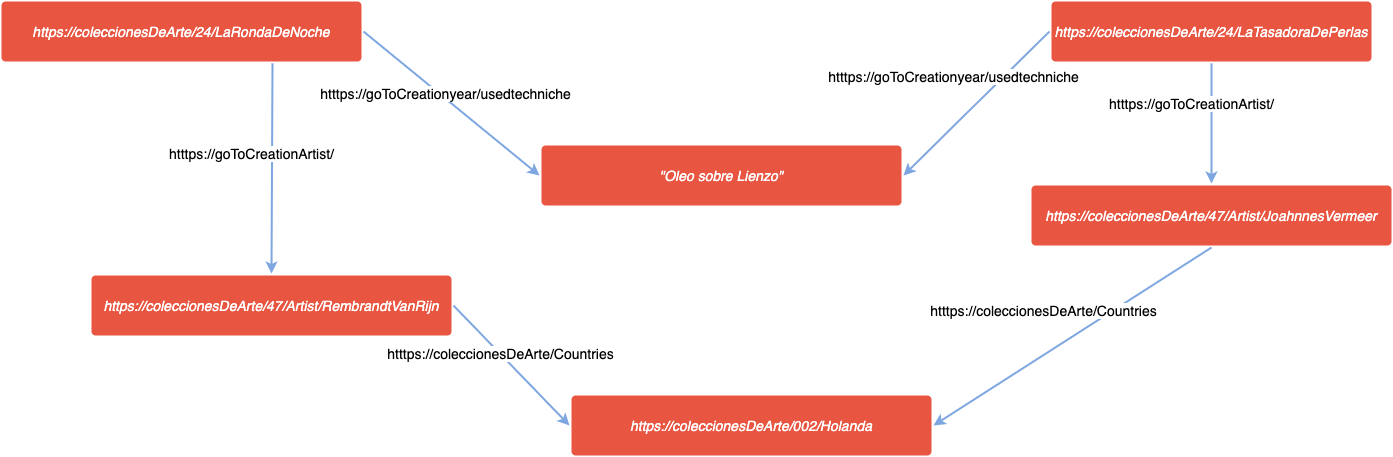
\includegraphics[width = 1\textwidth]{Imagenes/Bitmap/RDFexample.png}
	\caption{Ejemplo de grafo siguiendo el modelo RDF}
	\label{fig:sampleImage}
\end{figure}

Para una persona normal, esta puede resultar una nomenclatura poco amigable ya que las URIs pueden llegar a ser mucho más engorrosas y complejas. Más adelante explicaremos cómo hemos resuelto este problema en nuestro proyecto para que cualquiera que haga uso de nuestra interfaz pueda reconocer todos los objetos y, sobre todo, para darnos mucha más comodidad a la hora de trabajar con ellos.\\

Podríamos decir que estamos estableciendo una relación entre dos objetos unidos mediante una propiedad. Esta propiedad es una ``explicación'' que nos sirve para relacionar objetos. En nuestro proyecto, estos objetos son canciones.\\


\section{Herramientas con uso de Linked Data}

Para poder trabajar con datos enlazados en la web, estos tienen que estar almacenados en los formatos previamente explicados, es decir, si queremos poder hacer consultas de obtención de datos enlazados a un servidor, este debe mantener internamente un formato RDF con todas las condiciones que ello implica. Actualmente existen diversos puntos para ello.\\

En nuestro caso, hay diversas plataformas que brindan este servicio. Se trata de un concepto que está creciendo enormemente y cada vez más empresas están adoptando este modelo de datos. En lo que la web se refiere, hay varios ejemplos los cuales hemos podido utilizar que tuviesen datasources con un contexto multimedia relacionado con temas musicales. Nosotros hemos optado por utilizar Wikidata, una base de datos muy similar a DBpedia que explicaremos a continuación.


\begin{figure}[h!]
	\centering
	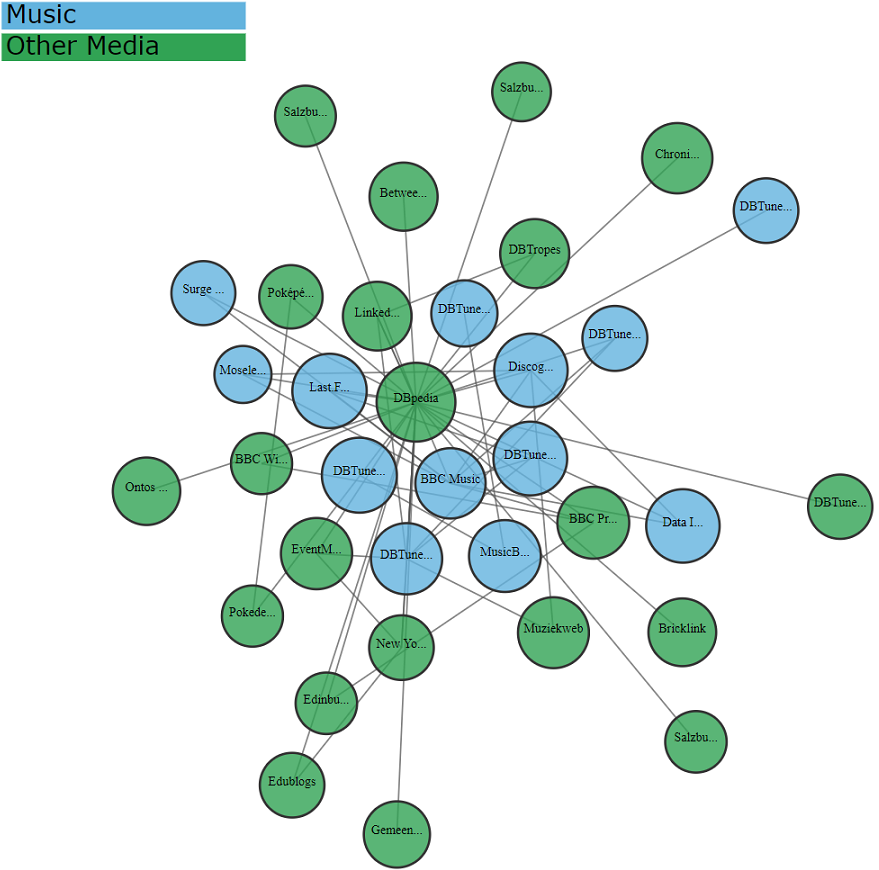
\includegraphics[width = 1\textwidth]{Imagenes/Bitmap/WIkis.png}
	\caption{Diagrama de datasets publicados con un formato linked data sobre contenido multimedia}
	\label{fig:sampleImage}
\end{figure}


\subsection{WikiData}

Wikidata es una base de datos libre, colaborativa, multilingüe y secundaria, que recopila datos estructurados para dar soporte a Wikipedia, Wikimedia Commons, así como a otras wikis del movimiento Wikimedia y a cualquier persona en el mundo \cite{wikidataIntro}. El proyecto comenzó en 2012 liderado por Wikimedia Alemania. Gracias a Wikidata, tenemos una gran cantidad de información relevante acerca de toda nuestra cultura reunida en un mismo sitio. La usaremos para consultar e investigar la información relacionada con nuestro dataset (o conjunto de datos), esencialmente datos acerca de artistas y sus temas musicales. Tiene numerosos servicios, uno de los que probablemente hayamos usado y no nos hemos dado cuenta, es el de servir información para rellenar las fichas de los artículos de Wikipedia.\\

Como se podrá observar en la Figura~\ref{fig:wikidataPage}, una ficha de Wikidata contiene un conjunto de tuplas propiedad-identificador. Por ejemplo, en este caso se señala que la propiedad Género de la canción tiene un identificador Funk (entre otros). A su vez, al  identificador Funk le corresponderá un código que no es más que una URI que nos trasladará a la propia ficha de este tipo de género musical. Así es como se aplica este sistema enlazado de información en Wikidata.\\

\begin{figure}[h!]
	\centering
	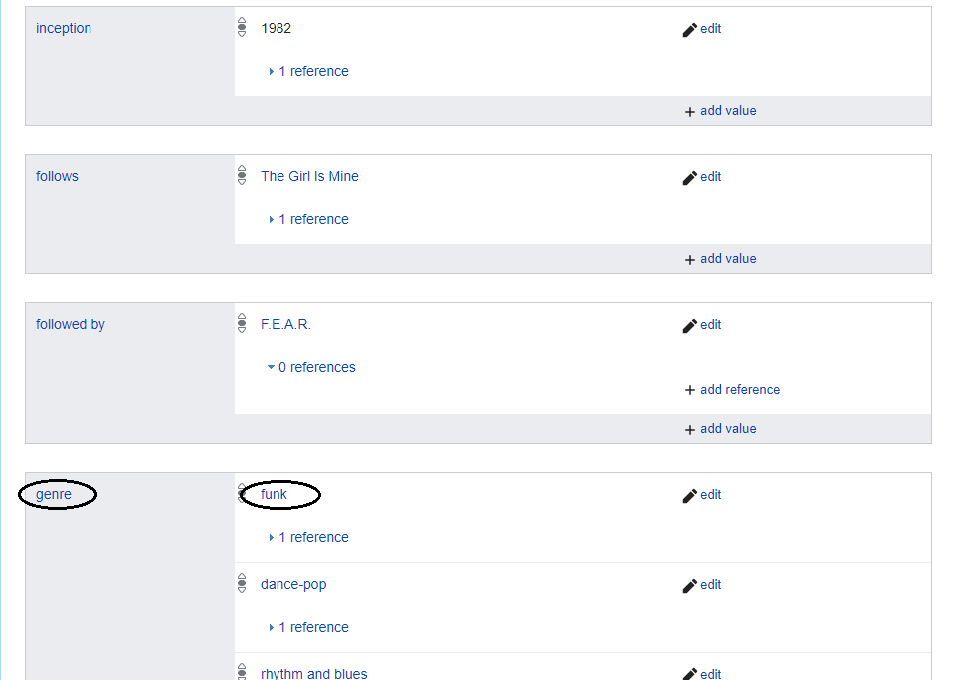
\includegraphics[width = 1\textwidth]{Imagenes/Bitmap/WikidataEx.png}
	\caption{Ejemplo de una página de Wikidata sobre la canción Billie Jean}
	\label{fig:wikidataPage}
\end{figure}

Wikidata está estructurada de tal manera que resulta sencillo acceder a su información utilizando el lenguaje de consultas SPARQL. Cada objeto tiene ciertas propiedades a las que podemos acceder seleccionando el identificador correcto de la propiedad.\\

Una de las ventajas de Wikidata es que nos va a eliminar toda la nomenclatura de URIs propias de SPARQL. En estas consultas, las entidades serán referenciadas con los caracteres wd y las propiedades con los caracteres wdt. Un ejemplo de una consulta sencilla podría ser:\\

-Obtén todos los Artistas cuyo género musical sea Rock:\\
\begin{lstlisting}[language=SPARQL]
SELECT ?singer ?singerLabel ?genre ?genreLabel
WHERE
{
	?singer wdt:P31 wd:Q215380;
	wdt:P136 wd:Q7749;
	SERVICE wikibase:label { bd:serviceParam wikibase:language &quot;en&quot; . }
}
\end{lstlisting}
\bigskip

En esta consulta estamos accediendo a todos los objetos que contengan las propiedades~(wdt) P31~(Tipo Instancia) y P136~(Género) con el valor~(wd) que nosotros estamos seleccionando, Q215380 y Q7749, forzando así a que las dos propiedades sean Grupo Musical y Rock and Roll respectivamente.\\

SPARQL es un lenguaje muy potente que puede abarcar gran cantidad de datos en función de la web (se pueden crear consultas mucho más complejas para obtener datos más específicos).


\subsection{SPARQL}

Finalmente, para poder empezar a trabajar con la información hemos usado el lenguaje SPARQL, el cual nos permite consultar los datos enlazados de la web. Este es un lenguaje especializado para buscar y consultar datos RDF. Básicamente facilita el acceso a las URIs para después poder aplicar todo tipo de selección de datos, restricciones, condiciones y límites a las entidades con los esquemas explicados anteriormente. La estructura de una consulta SPARQL suele ser la siguiente:\\

\begin{lstlisting}[language=SPARQL]
PREFIX EX: Uri de una web
SELECT * variables que se desean conseguir
WHERE
{
	Operaciones con tripletas
}
OFFSET X intervalo de desplazamiento
LIMIT X limite de los datos obtenidos
\end{lstlisting}
\bigskip

La cadena PREFIX hace referencia a la URI o URIs donde se encuentran localizados las entidades a las que hacen referencia las tripletas. Su objetivo es no tener que escribir la URI entera, la cual es una cadena de texto poco amigable para un usuario, cada vez que lo referenciáramos en una relación de las tripleta dentro de la cláusula WHERE.\\

A la hora de hacer una consulta compleja, es posible que lleguemos a un código que referencie muchas URIs y entidades de forma que no sea un lenguaje de uso fácil. Es por esto por lo que pudimos encontrar variedad mediante la librería que nos dispone Wikidata que simplifica algo más la nomenclatura y los caracteres de este lenguaje.\\


%\chapter{Tecnologías y Herramientas utilizadas}
\label{cap:tecnologias}

\section{Programación}

\subsection*{Python}

Ha sido el lenguaje de programación principal, al menos en la parte del back end tanto para el núcleo del código que obtiene y relaciona los datos como para la creación de distintos scripts de ayuda, además de numerosas funciones para tratar los datos a representar en los grafos finales. Lo hemos escogido debido a su versatilidad y a su gran adaptación debido a la cantidad de librerías con las que cuenta.

\subsection*{Pandas y Numpy}

Dos librerías propias de Python, especializadas en el manejo y procesamiento de datos. Han sido de una utilidad vital ya que en gran parte del trabajo trabajamos con numerosos datasets y estas librerías nos proporcionan todo lo necesario para tratarlos, pudiendo así trabajar con ellos más fácilmente.

\subsection*{HTML y CSS}

Dos lenguajes fundamentales para la programación web. Debido a la naturaleza de nuestra aplicación hemos recurrido a estos lenguajes para darle forma y estilo a la interfaz de explicaciones, aquella parte de nuestro proyecto con la que interactuarán los usuarios.

\subsection*{Javascript}

Al igual que los anteriores, este es un lenguaje de programación muy importante para el desarrollo web. Javascript es una parte integral de nuestro proyecto, pues es el lenguaje en el que se ha desarrollado la parte encargada de dibujar los grafos de explicaciones, además de otras funciones necesarias para el funcionamiento de la interfaz.

\subsection*{vis.js}

Esta es una librería de Javascript para visualización de datos. Permite diversas representaciones gráficas, pero nosotros hemos empleado el componente Network para dibujar nuestros grafos de explicaciones. Es una librería bastante completa y con una documentación bien organizada, así que fue muy útil a la hora de plasmar en pantalla el resultado de nuestra investigación.

\subsection*{Jupyter-Notebooks}

Es un entorno informático interactivo basado en la web. Fue un entorno apropiado para realizar la prueba de scripts que nos ayudaron a limpiar y probar el dataset original.

\section{Organización}

\subsection*{Github}

Para poder almacenar y organizar todo el código en el que hemos trabajado conjuntamente. Nos ha permitido llevar un historial de versiones y actualizaciones de cada módulo del código. Github ha sido una herramienta apropiada no solo para llevar un control del código de la aplicación, sino también para la construcción de este mismo documento.

\subsection*{Google Drive}

Empleamos el servicio de alojamiento de archivos en la nube de Google para recoger y poner en común todos los documentos relacionados con la investigación previa al inicio del trabajo, además de para compartir recursos durante la realización del mismo. Su importancia quedó relegada a un segundo plano a medida que avanzaba el proyecto debido a que comenzamos a utilizar Github, pero cabe resaltar su utilidad durante las primeras fases.

\subsection*{Google Meet}

La aplicación de videoconferencias de Google fue una herramienta clave para mantener el contacto tanto con los directores del TFG como entre los miembros del equipo. Cuando las reuniones presenciales dejaron de ser posibles por motivos ajenos a nuestro control, se hizo necesario el uso de un servicio como este.

\section{Memoria}

\subsection*{LaTeX}

Este ha sido el procesador de textos elegido para la realización de este documento: la Memoria del TFG. Nos decantamos por este en lugar de otros procesadores como Word debido a las muchas posibilidades que tiene para generar documentos de calidad. Puntos como la estructura de capítulos, la estandarización de títulos o la forma de mostrar figuras (tanto imágenes como fragmentos de código), han hecho que nos resulte más sencilla la tarea de desarrollar esta memoria.

\subsection*{TeXiS}

TeXiS es una plantilla de LaTeX para Tesis, Trabajos de Fin de Máster y otros documentos desarrollada por Marco Antonio y Pedro Pablo Gómez Martín. Es la plantilla que se ha usado como base para construir este documento y ha resultado de gran ayuda tanto para cuestiones de organización como para aprender a usar varias funcionalidades de LaTeX, lo cual ha sido muy importante debido a nuestra falta de experiencia previa a este proyecto.

\section{Tecnologías y herramientas descartadas}

\subsection*{Alchemy.js}

Alchemy.js es una aplicación de visualización de grafos para la web. Está escrita en JavaScript con la librería D3.js como base y ofrece una manera sencilla y rápida de generar grafos. La mayoría de su personalización se lleva a cabo sobrescribiendo sus configuraciones por defecto, por lo que no requiere apenas implementar código JavaScript adicional.\\

Fue la primera opción contemplada para representar los grafos de nuestro proyecto debido a su sencillez de manejo y a su uso de archivos JSON para aportar los datos, algo que resultaba atractivo en un principio. Tras trabajar con ella durante un tiempo fue necesario descartarla por ciertas limitaciones a la hora de personalizar la representación según nuestro diseño, además de la falta de soporte por tratarse de un proyecto actualmente abandonado.
\chapter{Explicaciones}
\label{cap:explicaciones}

El objetivo de nuestro trabajo consiste en explicar las relaciones entre dos canciones dadas por un recomendador de música que trabaja con un dataset concreto. De esta manera, llamaremos \textbf{explicación} a cada factor común que compartan ambas canciones, siendo principalmente propiedades que poseen las propias canciones o los valores de otras propiedades intermedias. A lo largo de este capítulo concretaremos todas las explicaciones que vamos a estudiar y el sistema que une todas ellas para poder relacionar dos canciones en su totalidad.\\

Las relaciones que recogemos en cualquier caso de uso forman un grafo siguiendo el modelo RDF. Hemos decidido, además de seguir ese formato, dotarlas de un nivel que escala a medida que el estudio se aleje del objeto canción inicial. Al expresar alejamiento, nos referimos a que, como en el contexto del formato RDF y Linked Data, la creación de relaciones se establece navegando por distintos objetos relacionados con el inicial secuencialmente. La idea de los niveles viene dada por dos motivos:\\

El primero es debido a la cercanía de niveles. Cuanto menor sea el nivel, significará que está mas próximo al objeto canción inicial y por ello tendrá más peso a la hora de relacionarlas.\\

El segundo es porque a la hora de representar gráficamente todas las relaciones, queremos dividirlas por objetos de estudio de una forma nivelada y ordenada.\\

En una primera fase, generaremos explicaciones básicas para relacionar directamente las dos canciones u objetos principales, por ejemplo: género, artista, álbum, etc. Asignaremos una complejidad de k=1 a las explicaciones directas. Estas explicaciones son una relación directa entre dos canciones relacionadas por una propiedad, es decir, solo tenemos en cuenta propiedades ligadas a cada objeto en un primer nivel.\\

Una vez obtenemos las relaciones básicas, es necesario seguir avanzando en el estudio, ya que dos canciones que a priori no son muy similares musicalmente, no compartirán casi ninguna de estas relaciones directas. Es por esto por lo que indagamos más en la información que podemos obtener a partir de las relaciones que hemos sacado en el paso anterior. Aquí aparecen las relaciones indirectas, aquellas que surgen del estudio de otras obtenidas en niveles anteriores, siempre que coincidan en ambas canciones. La idea es poder representar toda la información compartida, de forma que se pueda representar con un grafo. Estas explicaciones pueden tener un nivel de complejidad diferente (k= 2, 3, 4...) dependiendo de cuántos niveles se hayan estudiado. La idea principal es ejecutar un estudio de ambas canciones obteniendo varios niveles de cada una de ellas, para finalmente unirlas enlazando únicamente las que coincidan.\\

Hemos recopilado a lo largo de investigación y consultas un conjunto de posibles relaciones a obtener, que suman un total de 24 explicaciones. Es importante añadir que la mayoría de ellas pueden presentarse en distintos niveles. Para explicar este caso más fácilmente lo representamos con el ejemplo de la Figura 3.1.\\


\begin{figure}[h!]
	\centering
	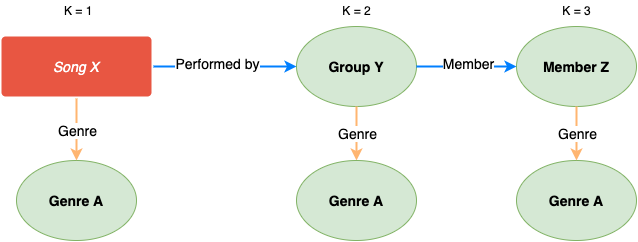
\includegraphics[width = 0.9\textwidth]{Imagenes/Bitmap/RelationLevels.png}
	\caption{Ejemplo de misma relación en distintos niveles}
	\label{fig:sampleImage}
\end{figure}

Para nuestro caso, en el cual tratamos con dos objetos iniciales que representan a dos canciones, hemos seleccionado una serie de propiedades a investigar para obtener los distintos niveles. El primer nivel es el más intuitivo: obtener relaciones directamente de ambas canciones. Entre esas relaciones se encontraría la relación ``Interpretado por'', la cual nos proporciona el artista o grupo que interpreta la canción. Este artista es el que vamos a usar como objeto de estudio del nivel k = 2, obteniendo así otro conjunto de relaciones del artista y sus respectivos valores. También obtendremos el género de la canción, que usaremos para generar el nivel k = 3 mediante las propiedades que obtengamos del género. Por último, como nivel final hemos seleccionado investigar las propiedades de los miembros que conforman la banda de música en caso de que el intérprete de la canción esté formado por varios artistas, y denominamos a este último nivel k= 4.\\

Queremos señalar que estos niveles podrían alargarse más a medida que seguimos investigando nuevas propiedades y generando un grafo más completo. Hemos decidido poner un límite en este punto debido a que, a medida que vamos avanzando en el estudio de los niveles de las propiedades, las explicaciones son menos significativas debido a que están más alejadas del primer nivel, que es el que está relacionado con la canción en sí.\\

En esta sección vamos a recopilar las principales propiedades de la lista total y cómo relacionarían dos canciones objeto iniciales. Algunas de ellas podrán aparecer en distintos niveles mientras que otras serán propias de un solo nivel:\\

\section{Explicaciones de la canción}

Aquí se encuentran las explicaciones basadas en propiedades del objeto canción que no pueden aparecer en el resto de niveles:

\subsection*{Artista}

El artista es una de las explicaciones más obvias pero también es una de las más importantes. Esta explicación hace referencia a cuando dos temas son interpretados por el mismo artista, por lo que tienen una clara relación directa ya que suele existir similitud entre las canciones de un artista. Además, a partir del artista podemos obtener otras relaciones más complejas en función de los datos de este mismo.\\

Como ejemplo podemos tomar los temas \textit{One More Time} y \textit{Something About Us}. Ambos son interpretados por el dúo musical \textbf{Daft Punk}, así que podemos explicar su relación gracias a este dato.\\

Para esta explicación utilizamos la propiedad ``performer''~(intérprete) de Wikidata. Siguiendo el modelo RDF, el sujeto es la canción (\textit{One More Time}, por ejemplo), el predicado es la propiedad intérprete y el objeto es el artista (\textbf{Daft Punk}).\\

\begin{figure}[h!]
	\centering
	
\includegraphics[width = 0.9\textwidth]{Imagenes/Bitmap/Artista ejemplo.png}
	\caption{Ejemplo de explicación por artista}
	\label{fig:sampleImage}
\end{figure}

\subsection*{Álbum}

Una explicación muy potente será que ambas canciones pertenezcan al mismo álbum. A menudo esta explicación aparecerá acompañada de la explicación del artista y, en cualquier caso, la relación que existe entre dos temas del mismo álbum suele ser más estrecha debido a que poseen más puntos en común, como puede ser el género, la fecha o la temática.\\

Tomemos como ejemplo \textit{Today} y \textit{Disarm}. Estas dos canciones son muy cercanas porque tienen varios puntos en común, pero una de las explicaciones que podemos ofrecer es que ambas pertenecen al álbum \textit{Siamese Dream}, de \textbf{The Smashing Pumpkins}. \textit{1979} es otro tema que se podría recomendar a raíz de \textit{Today}, pero es una peor elección que \textit{Disarm} porque pertenece a un álbum diferente.\\

Volvemos a utilizar Wikidata para obtener esta explicación, concretamente la propiedad ``part of''~(parte de). Esta propiedad se utiliza para varias cosas, entre ellas indicar los álbumes a los que pertenecen las canciones. Así obtenemos que \textit{Today} es ``parte de'' \textit{Siamese Dream}.\\

\begin{figure}[h!]
	\centering
	
\includegraphics[width = 0.9\textwidth]{Imagenes/Bitmap/Álbum ejemplo.png}
	\caption{Ejemplo de explicación por álbum}
	\label{fig:sampleImage}
\end{figure}

\subsection*{Fecha de publicación (Década)}

Creemos que hay una mayor probabilidad de que exista una relación entre dos canciones que pertenezcan a la misma década. Esto se debe a que a lo largo del tiempo ha habido periodos marcados por uno o varios géneros musicales. Esto también ayuda a estudiar cómo estos distintos géneros están relacionados entre sí, lo cual es otro punto importante a tener en cuenta ya que hay géneros íntimamente relacionados entre sí: techno y house, heavy metal y thrash metal, etc.\\

Gracias a esta explicación, podemos relacionar dos canciones que a priori son muy distintas, como es el caso de \textit{September} de \textbf{Earth, Wind \& Fire} y \textit{Bohemian Rhapsody} de \textbf{Queen}. Estos temas no comparten algo tan básico como el artista o el género, pero ambos fueron publicados en los años 70 y por ello pueden resultar interesantes para un usuario que busque escuchar los ritmos de esa época.\\

Para obtener esta explicación, emplearemos la propiedad ``publication date''~(fecha de publicación) de las canciones en Wikidata y comprobaremos si las dos fechas se sitúan dentro de la misma década.\\

\begin{figure}[h!]
	\centering
	\includegraphics[width = 0.9\textwidth]{Imagenes/Bitmap/Década ejemplo.png}
	\caption{Ejemplo de explicación por década}
	\label{fig:sampleImage}
\end{figure}

\subsection*{Singles}

Existe también una cierta relación entre aquellos temas que sean singles (o sencillos), así que consideramos esto como una explicación más. El razonamiento para esta decisión es que los singles son canciones que se publican de forma independiente por razones promocionales, por lo que suelen convertirse en los temas más populares y representativos del trabajo del artista. Por ello, pueden poseer más valor para el recomendador que otras canciones porque los singles tienen más probabilidades de coincidir con los gustos del usuario.\\

El tema \textit{Hung Up} de \textbf{Madonna} es un single, así que podemos establecer cierta relación con \textit{Feel Good Inc.} de \textbf{Gorillaz}, que también es un single.\\

Para esta explicación emplearemos la propiedad ``instance of''~(instancia de) en Wikidata y su valor ``single''. De esta forma comprobaremos que tanto \textit{Hung Up} como \textit{Feel Good Inc.} son ``instancia de'' ``single''.\\

\begin{figure}[h!]
	\centering
	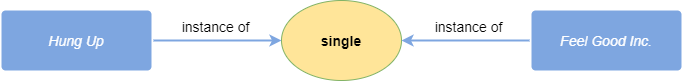
\includegraphics[width = 0.9\textwidth]{Imagenes/Bitmap/Single ejemplo.png}
	\caption{Ejemplo de explicación por single}
	\label{fig:sampleImage}
\end{figure}

\section{Explicaciones compartidas por Artista y Canción}

En esta sección exponemos propiedades que pueden ser establecidas tanto en el nivel de estudio de la canción como en el nivel de estudio del artista.

\subsection*{Premios}

La siguiente explicación son los premios recibidos. Existe una variedad de premios compartidos por diferentes canciones. Algunos de estos premios son más específicos que otros, pero en cualquier caso pueden resultar una relación útil para nuestras explicaciones ya que son un reflejo de la repercusión de las canciones. El mismo caso se da para los artistas, aquellos que suelen optar al mismo premio tienen más posibilidades de tener un estilo muy similar y por ende se puede establecer una relación de cercanía.\\

En esta sección hemos recogido dos propiedades: ``award received''~(premio recibido) y ``nominated for''~(nominado a). Estas categorías hacen referencia a los premios que han recibido los artistas o canciones y a los premios a los que han sido nominados respectivamente. Normalmente los premios se reparten según distintas categorías en función al estilo de música, pero también hay otros que nos aportan otro tipo de información al estudio como Grammy al Mejor Videoclip, Grammy Award a la Mejor Canción Escrita, Grammy Award a la Mejor Interpretación Rap/Sung etc...\\

Basándonos en el nivel de canción tenemos como ejemplo \textit{Single Ladies (Put a Ring on It)} de \textbf{Beyoncé} y \textit{Rolling in the Deep} de \textbf{Adele}, ya que ambos temas han recibido el Premio Grammy a la canción del año. Además, como es lógico, ambas canciones fueron nominadas a ese mismo premio, así que podemos mostrar ambas propiedades en este ejemplo.\\

Usaremos la propiedad ``award received''~(premio recibido) y ``nominated for''~(nominado a) encontradas en Wikidata. De esta forma, \textit{Rolling in the Deep} sería el sujeto, ``award received'' y ``nominated for'' serían los predicados y \textit{Grammy Award for Song of the Year} sería el objeto.\\

\begin{figure}[h!]
	\centering
	
\includegraphics[width = 0.9\textwidth]{Imagenes/Bitmap/Premio ejemplo.png}
	\caption{Ejemplo de explicación por premio}
	\label{fig:sampleImage}
\end{figure}

\subsection*{Género}

La explicación Género es una de las más representativas ya que las personas se guían por el género que prefieren para escuchar canciones similares, aunque en ocasiones no deba ser así. Un usuario que sea fan del jazz querrá escuchar canciones de ese mismo género o géneros similares porque todas los temas de un mismo género comparten una serie de puntos en común como la elección de los instrumentos, temáticas similares en sus letras o patrones de composición.\\

Gracias al género, podemos explicar la relación entre canciones como \textit{Master of Puppets} de \textbf{Metallica} e \textit{Indians} de \textbf{Anthrax}, que pertenecen al \textbf{thrash metal}.\\

Para esta relación utilizamos la propiedad ``genre''~(género) de Wikidata. Así tenemos que la canción \textit{Master of Puppets} pertenece al género \textbf{thrash metal}.\\

\begin{figure}[h!]
	\centering
	\includegraphics[width = 0.9\textwidth]{Imagenes/Bitmap/Género ejemplo.png}
	\caption{Ejemplo de explicación por género}
	\label{fig:sampleImage}
\end{figure}

En este caso podríamos crear la misma relación con los artistas, debido a que ambos artistas de las dos canciones previas también cuentan con un registro de thrash metal (entre otros géneros) en su propiedad de género.\\

\subsection*{Idioma}

La explicación Idioma denota, como su nombre sugiere, que ambas canciones están en el mismo idioma o lenguaje. Existen numerosos ejemplos de temas musicales que están escritos en un idioma que no se corresponde con la lengua materna del artista que los publican, o sencillamente están escritas en un idioma que se habla en varias partes del mundo distintas, como el inglés o el español. En ciertos casos el compartir idioma es un indicativo de otras relaciones adicionales, como puede ser el caso de canciones que pertenecen a un folclore regional determinado. En cualquier caso el compartir lenguaje ya es una relación directa en sí misma.\\

Como ejemplo podemos tomar el tema \textit{Like a Virgin} de \textbf{Madonna} y \textit{Rocket Man} de \textbf{Elton John}, los cuales están escritos en inglés.\\

Para esta explicación emplearemos la propiedad ``language of work or name''~(idioma de la obra o del nombre) de Wikidata. Así tenemos que la canción \textit{Like a Virgin} tiene idioma ``inglés''.\\

\begin{figure}[h!]
	\centering
	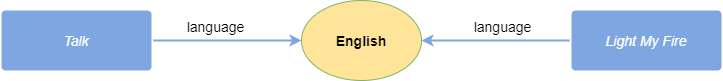
\includegraphics[width = 0.9\textwidth]{Imagenes/Bitmap/Idioma ejemplo.png}
	\caption{Ejemplo de explicación por idioma}
	\label{fig:sampleImage}
\end{figure}

El mismo caso podría servir de ejemplo para relacionar ambos artistas con la misma propiedad de idioma significando que ambas canciones son interpretadas en ese idioma.\\

\section{Explicaciones compartidas por Artista y Miembros}

En esta sección solo aparecen las principales propiedades que por naturaleza son exclusivas de un artista, ya sea un artista en solitario o un miembro del grupo.\\

\subsection*{Compañía discográfica}

Record Label~(compañía discográfica) hace referencia a la compañía por la que ha firmado el artista para publicar un tema concreto. Hemos podido observar que una misma compañía puede firmar a artistas que a veces no tienen relación ninguna en cuanto al estilo musical, pero hay otras causas que sí los pueden relacionar indirectamente como la tendencia del momento, el target del público que generan, etc. También se puede dar el caso en el que un miembro del grupo firme o haya firmado con una compañía individual, ya sea por conceptos relacionados con marcas, representantes o contratos.\\

Para ilustrarlo con un ejemplo, tanto la canción \textit{Born in the U.S.A.} de \textbf{Bruce Springsteen} como la canción \textit{Ashes} de \textbf{Céline Dion} fueron publicadas por el sello discográfico \textbf{Columbia Records}.\\

Podemos alcanzar esta explicación gracias a la propiedad ``record label''~(sello discográfico) de Wikidata. \textit{Born in the U.S.A.} tiene un ``record label'' cuyo nombre (o valor) es \textbf{Columbia Records}.\\

\begin{figure}[h!]
	\centering
	\includegraphics[width = 0.9\textwidth]{Imagenes/Bitmap/Discográfica ejemplo.png}
	\caption{Ejemplo de explicación por compañía discográfica}
	\label{fig:sampleImage}
\end{figure}

\subsection*{Lugar de formación}

La propiedad ``location of formation''~(lugar de formación) que hace referencia a la localidad de formación del grupo o artista, puede parecer muy similar a la explicación ``country of origin'', pero esta ejerce una selección más precisa porque nos da un núcleo de población más pequeño. Un ejemplo de ello podrían ser dos míticas bandas de la ciudad de Boston: Aerosmith y Boston. Creemos que la unión de la ciudad natal con la música puede hacer a un usuario el escuchar grupos de su misma ciudad o estado. En cuanto a la relación referente a un miembro del grupo, se trataría del lugar donde ese miembro se inició como músico ya sea como artista en solitario o en su grupo original.\\

\begin{figure}[h!]
	\centering
	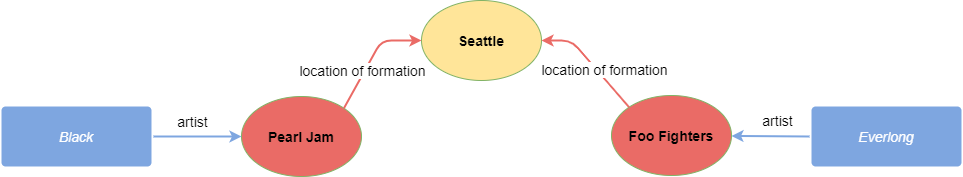
\includegraphics[width = 0.9\textwidth]{Imagenes/Bitmap/LocationOfFormation.png}
	\caption{Ejemplo de explicación por lugar de formación}
	\label{fig:sampleImage}
\end{figure}

\section{Explicaciones compartidas por Artista, Miembro, Género y Canción}

Estas explicaciones son compartidas en los cuatro niveles y resultan de gran interés porque nos permitirán enlazar los cuatro mismos en el caso en el que coincidan en el objeto con las relaciones de la canción opuesta.\\

\subsubsection*{País de origen}

Esta explicación puede ser especialmente útil para países relativamente pequeños donde la música nacional presenta unos patrones claros. Además, a lo largo de la historia en un país se genera una tendencia o nuevo género musical el cual es propio de ese país en el que se forma un artista y esto nos daría una relación muy específica que definitivamente acertaría por completo en la relación 1 a 1 de dos canciones.\\

En países que son significativamente grandes o con una población muy alta perdería algo de especificidad, pero aún así hay más posibilidades de que dos un artistas del mismo país sean escuchados por un mismo usuario.\\

La canción \textit{Fire} de la banda \textbf{BTS} y \textit{Kill This Love} de \textbf{Blackpink} guardan cierta similitud porque ambos grupos son originarios de \textbf{Corea del Sur}.\\

Para comprobarlo, obtendremos la propiedad ``country of origin''~(país de origen) del artista que previamente ya hemos almacenado al estudiar las relaciones directas en el caso de las bandas o la propiedad ``country of citizenship''~(país de nacionalidad) en el caso de los artistas en solitario. \textit{Fire} tiene el ``performer'' \textbf{BTS}, cuyo ``country of origin'' es Corea del Sur.\\

\begin{figure}[h!]
	\centering
	\includegraphics[width = 1\textwidth]{Imagenes/Bitmap/País ejemplo.png}
	\caption{Ejemplo de explicación por país de origen}
	\label{fig:sampleImage}
\end{figure}

También podemos recoger la información del país donde se formó ese género. Con esta propiedad queremos recoger movimientos artísticos que surgieron en el mismo país. Los géneros que fueron formados en un determinado país están mucho más arraigados a este a pesar de que se hayan extendido por todo el mundo. Es por esto que si queremos relacionar una artista que cualquier parte del mundo, que tiene un estilo techno, será más propenso a estar relacionado con artistas o canciones holandesas, cuna de este estilo musical.\\

En el caso de que la propiedad se estableciese en la canción, significaría que ambas canciones han sido lanzadas originariamente en el mismo país.\\

\subsubsection*{Influenciado por}

La \textbf{influencia de los artistas} es otra explicación importante. A menudo el trabajo de un artista se ve influenciado por otros artistas de formas que no siempre están ligadas a un género musical concreto, así que podemos encontrar una relación entre dos canciones examinando estas influencias.\\

Tomando como ejemplo las canciones \textit{Billie Jean} de \textbf{Michael Jackson} y \textit{Paint It Black} de \textbf{The Rolling Stones}, podemos establecer una relación entre ellas al ver que ambos artistas fueron influenciados por la banda \textbf{The Beatles}.\\

Obtenemos esta explicación gracias a la propiedad ``influenced by''~(influenciado por) de Wikidata, además de la propiedad ``performer'' para relacionar el tema con su artista. Así averiguamos que \textit{Billie Jean} tiene de ``intérprete'' a \textbf{Michael Jackson}, quien fue ``influenciado por'' \textbf{The Beatles}.\\

\begin{figure}[h!]
	\centering
	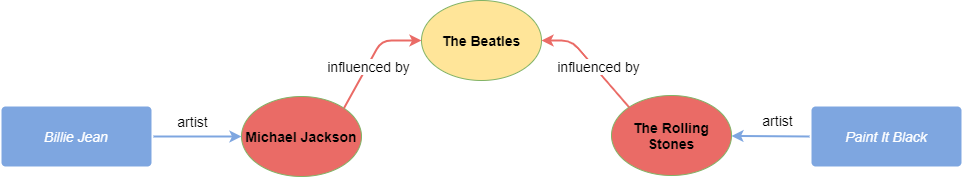
\includegraphics[width = 1\textwidth]{Imagenes/Bitmap/Influencia ejemplo.png}
	\caption{Ejemplo de explicación por influencia}
	\label{fig:sampleImage}
\end{figure}

Al igual que con el artista, los géneros también son influenciados por otros los cuales ha servido para el desarrollo de nuevos estilos a lo largo de la historia. Gracias a la evolución del Rock hay otros géneros que han marcado tendencia como el Rock and Roll, el Heavy Metal,Hard Rock, Garage Rock etc...\\

\section{Propiedades propias del artista o grupo}

Aquí se expones las principales relaciones que solo pueden ser propias del artista o grupo.\\

\subsubsection*{Integrantes}

Los \textbf{integrantes} son cada uno de los miembros que conforman un grupo. En caso de ser un único artista, esta propiedad es irrelevante ya que haríamos referencia a la propiedad directa de artista. Esta propiedad resulta útil en casos en los que miembros de la banda han cambiado de grupo a lo largo de su carrera musical. Esto nos da acceso a otros grupos que por valores o gustos musicales del artista nos hacen pensar que pueden ser muy parecidos.\\

Si tomamos los temas \textit{Lithium} de \textbf{Nirvana} y \textit{The Pretender} de \textbf{Foo Fighters} podemos observar que existe una relación entre ellos porque el músico \textbf{Dave Grohl} ha formado parte de ambas bandas.\\

Para comprobarlo usaremos la propiedad de Wikidata ``performer'' y después comprobaremos la propiedad ``has part''~(compuesto de) para ver todos los miembros de la banda y buscar coincidencias. De este modo, podemos ver que \textit{The Pretender} tiene un ``performer'' que es \textbf{Foo Fighters}, y a su vez \textbf{Foo Fighters} ``has part'' \textbf{Dave Grohl}.\\\\\\

\begin{figure}[h!]
	\centering
	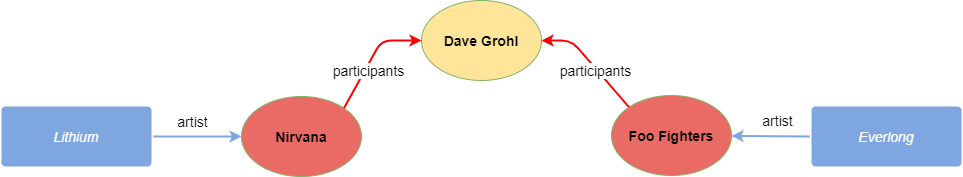
\includegraphics[width = 0.8\textwidth]{Imagenes/Bitmap/Integrante ejemplo.png}
	\caption{Ejemplo de explicación por integrantes}
	\label{fig:sampleImage}
\end{figure}

\subsubsection*{Tipo de voz}

Siguiendo con el estudio de los artistas, el \textbf{tipo de voz} de los vocalistas es una buena explicación para relacionar dos canciones. El tipo de voz influye en el sonido general del tema y puede ser especialmente determinante en ciertos géneros musicales. Por limitaciones técnicas, solo aplicaremos esta explicación con artistas en solitario.\\

La voz de un artista puede encajar en más de un tipo, como veremos en el siguiente ejemplo, aunque en esta explicación buscamos que coincidan en al menos un tipo. La cantante \textbf{Lady Gaga} se asemeja a \textbf{Amy Winehouse} por su tipo de voz, ya que ambas son \textit{mezzo-soprano} y \textit{contralto}. Así podemos explicar la relación entre dos canciones de estas artistas como \textit{Poker Face} y \textit{Rehab}.\\

Para esta explicación resulta útil la propiedad ``voice type''~(tipo de voz) en Wikidata. Partiendo de \textit{Poker Face}, utilizamos la propiedad ``performer'' para llegar a \textbf{Lady Gaga} y finalmente usamos su ``voice type'' para obtener \textit{mezzo-soprano}.\\

\begin{figure}[h!]
	\centering
	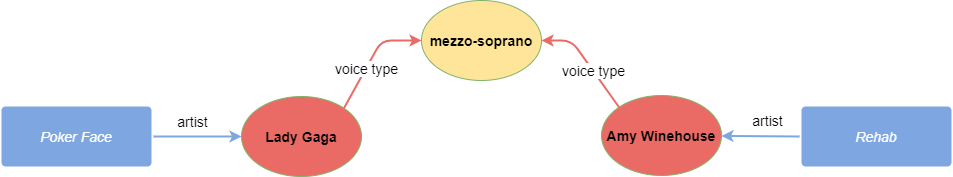
\includegraphics[width = 1\textwidth]{Imagenes/Bitmap/Voz ejemplo.png}
	\caption{Ejemplo de explicación por tipo de voz}
	\label{fig:sampleImage}
\end{figure}

\subsubsection*{Fecha de fundación}

Con esta propiedad intentamos tener en cuenta la historia de los o su cronograma. Hay grupos que comenzaron su etapa musical  conjuntamente a lo largo del tiempo. Un ejemplo de este caso se en curiosamente en el technopop que tanto caracterizó a los años 80, pues convivió a veces con el soul y con el estilo afroamericano doo-wop.\\

Gracias a esta explicación podemos relacionar canciones como \textit{Sweet Love} de \textbf{Anita Baker} y \textit{Musique Non-Stop} de \textbf{Kraftwerk}. Son canciones muy diferentes, pero ambos artistas comenzaron su carrera en la década de los 70, por lo que comparten un marco temporal.\\

Utilizaremos la propiedad ``work period (start)''~(inicio del periodo de actividad) de Wikidata para obtener esta explicación. \textit{Musique Non-Stop} tiene de intérprete a \textbf{Kraftwerk}, que a su vez inició su periodo de actividad en \textbf{1970}, es decir, en la década de los 70.\\

\begin{figure}[h!]
	\centering
	\includegraphics[width = 1\textwidth]{Imagenes/Bitmap/Fundación ejemplo.png}
	\caption{Ejemplo de explicación por fecha de fundación}
	\label{fig:sampleImage}
\end{figure}

\section{Explicaciones basadas en el género}

Estas propiedades vienen ligadas directamente al género de la canción. Es una de las propiedades más detalladas en Wikidata y por lo tanto una de de las que más información nos pueden proporcionar. Hay muchos géneros y subgéneros documentados, lo que nos facilita la obtención y clasificación de estos.\\

\subsection{Subgénero}

Cabe destacar la diferencia entre las propiedades ``Influed by''~(Influenciado por) y ``Subgenre''~(Subgénero); mientras que la primera solo indica que ese estilo musical ha marcado una cierta influencia tomando algunos aspectos, la segunda señala que es un Subgénero, una tendencia muy parecida y que toma como base ese estilo musical.\\

\begin{figure}[h!]
	\centering
	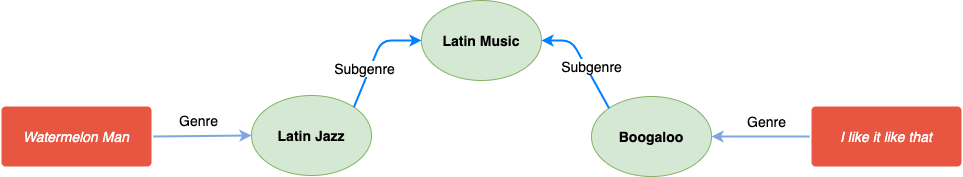
\includegraphics[width = 1\textwidth]{Imagenes/Bitmap/Subgenre.png}
	\caption{Ejemplo de explicación por Subgénero}
	\label{fig:sampleImage}
\end{figure}



\chapter{Diseño de la interfaz de explicaciones}
\label{cap:interfaz}

El objetivo de nuestro proyecto, como ya hemos expresado anteriormente en este documento, consiste en proporcionar explicaciones que justifiquen la relación existente entre dos canciones proporcionadas por un recomendador de música. Una vez realizado el estudio de las canciones y las distintas explicaciones posibles, es necesario mostrar el resultado de nuestro estudio de una forma gráfica, comprensible para un usuario humano.\\

Los datos que manejamos en nuestro estudio consisten en objetos y las relaciones que existen entre ellos, pues siguen el modelo de datos RDF. Necesitamos representar todos los caminos que se forman entre las dos canciones iniciales, mostrando las conexiones existentes entre los objetos intermedios. Por estos motivos hemos decidido llevar a cabo la visualización mediante un grafo porque consideramos que se adecúa mejor a nuestras necesidades.\\

Es importante que la interfaz sea fácil de entender y usar, así que siempre trataremos de mantenerla lo más sencilla posible. La base de nuestro diseño es el grafo de explicaciones ya mencionado, pues es el elemento más importante debido a la gran cantidad de información que aporta y, por lo tanto, es también la parte central de la interfaz alrededor de la cual se posicionarán el resto de elementos.\\

\section{Diseño del grafo}

\begin{figure}[h!]
	\centering
	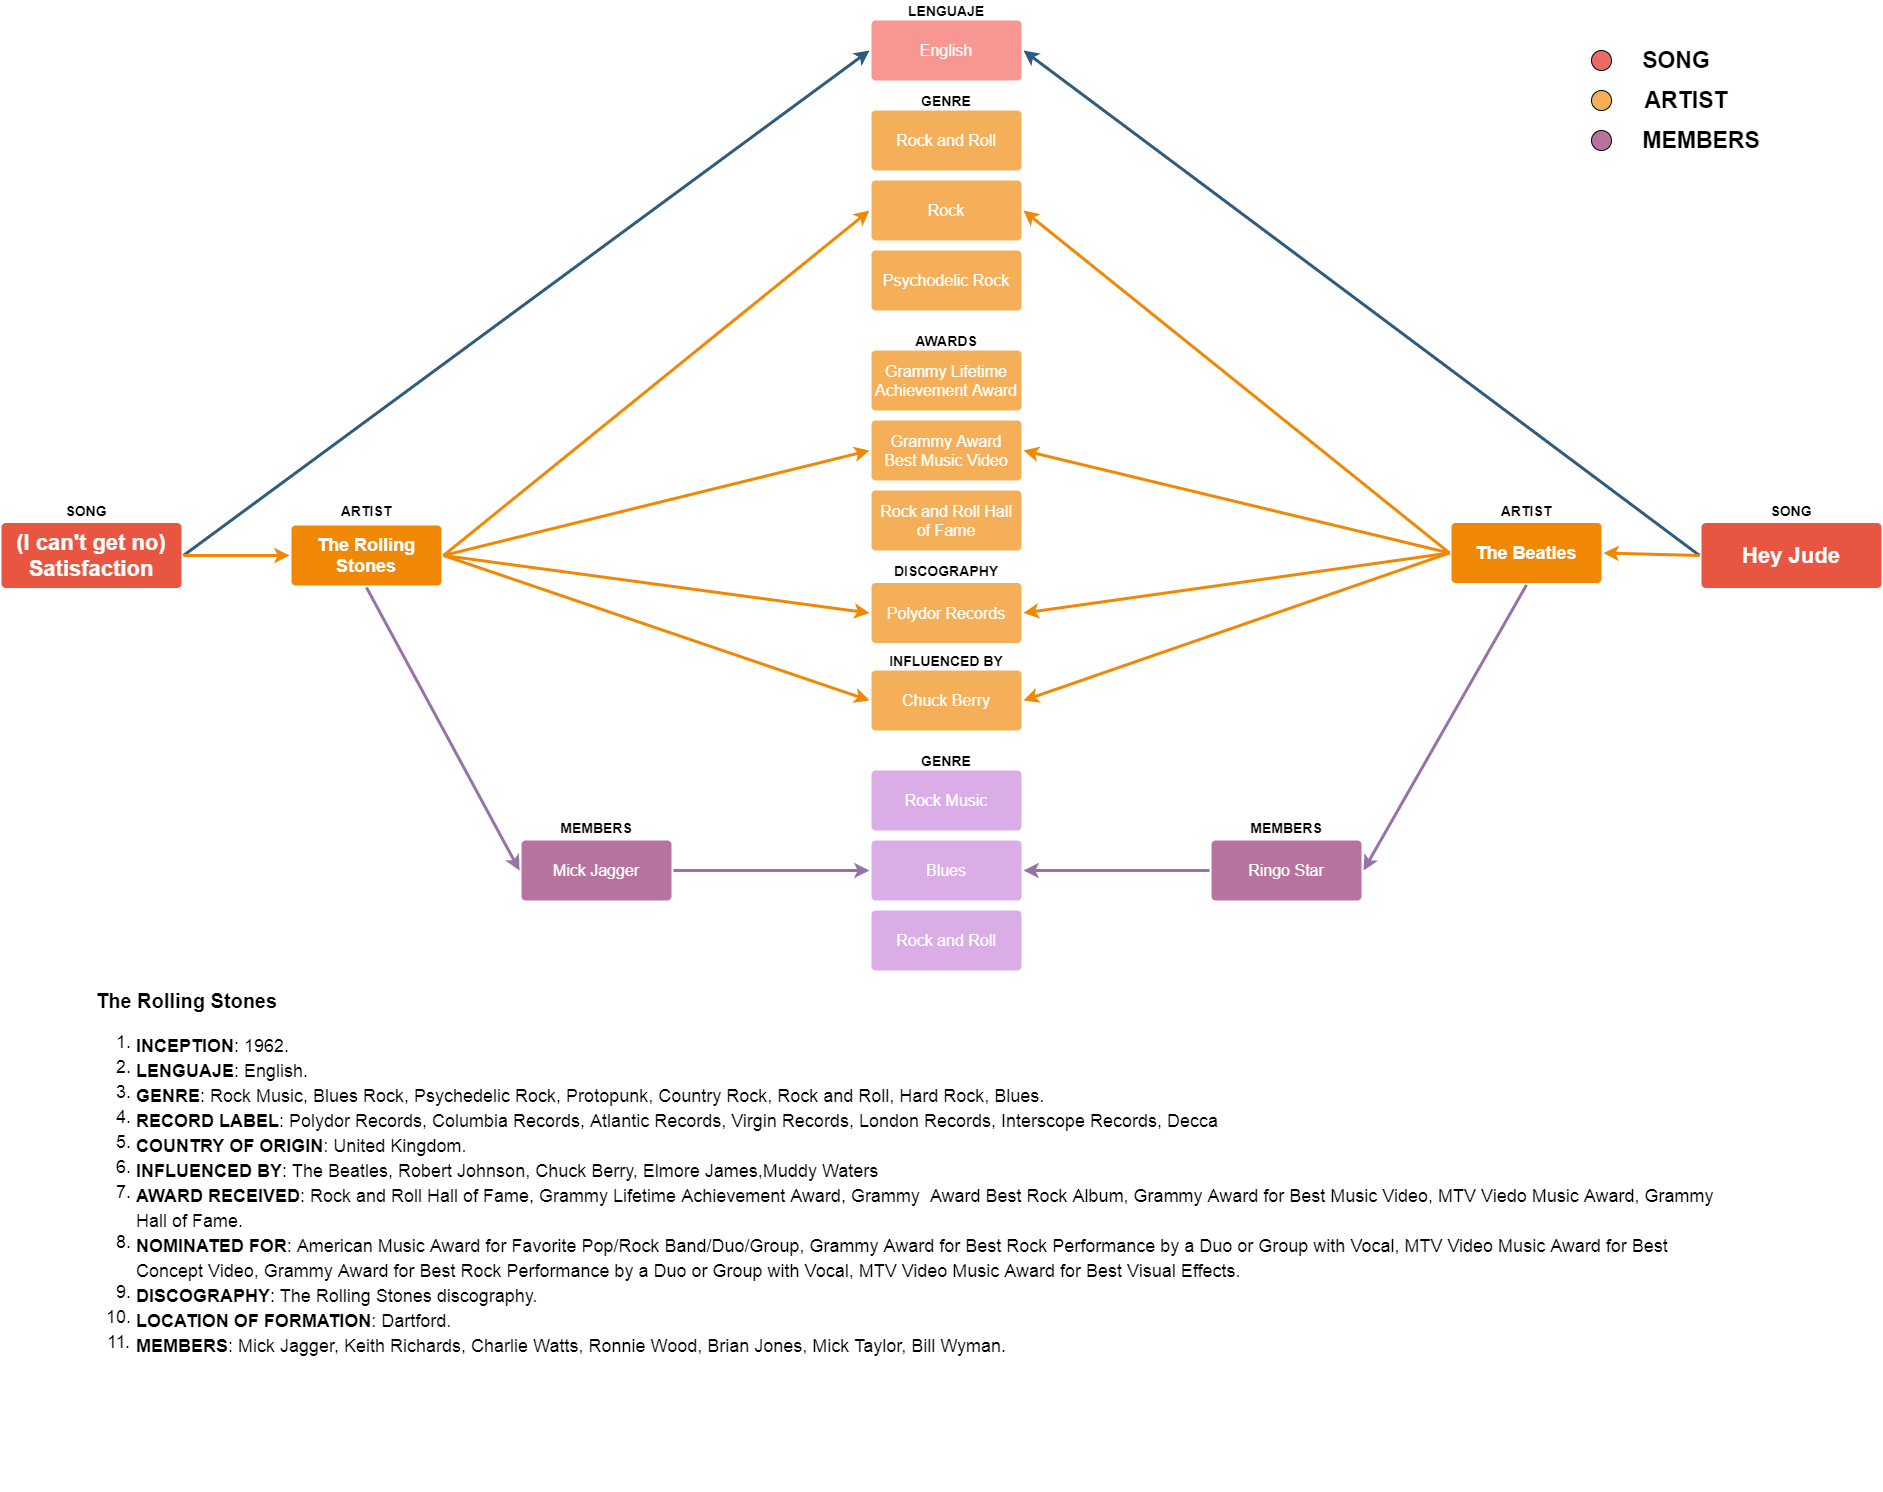
\includegraphics[width = 1\textwidth]{Imagenes/Bitmap/InterfaceResult.png}
	\caption{Primer diseño de la interfaz web}
	\label{fig:sampleImage}
\end{figure}

En la Figura 4.1 se puede observar la primera iteración de nuestro diseño. En ella se ve un ejemplo de grafo donde los nodos son los distintos sujetos y objetos (según el modelo RDF), mientras que las aristas representan los predicados que relacionan a esos nodos.\\

Los nodos posicionados a ambos extremos son las canciones sobre las que estamos realizando el estudio, diferenciados por el color rojo. A partir de ellas parten todas las explicaciones. En el centro se puede ver también un nodo coloreado de un rojo más suave, este representa al objeto de una explicación directa (en este caso la explicación ``Idioma'').\\

Los nodos coloreados de color naranja representan los artistas de ambas canciones y las relaciones que existen entre ellos, de la misma forma que en el anterior caso con las canciones y las explicaciones directas. Estas explicaciones obtenidas por el estudio de los artistas son indirectas, ya que requieren un estudio más profundo para relacionar las canciones originales.\\

Por último tenemos nodos morados que representan a los miembros o integrantes de los artistas, pues en este caso dichos artistas son bandas formadas por varias personas. Su funcionamiento es el mismo que el descrito en el párrafo anterior, con la salvedad de que estos miembros se obtienen del artista y, por lo tanto, sus explicaciones presentan un nivel extra de profundidad.\\

En esta versión del diseño también se propone una funcionalidad que permite visualizar datos adicionales. Haciendo click en los nodos sobre los que se hacen los estudios (canciones, artistas y miembros), se despliega una sección inferior en la que se muestran todos los datos obtenidos en el estudio del elemento concreto, aparezcan en el grafo o no. Así podemos ver todos los sellos discográficos con los que trabajaron \textbf{The Rolling Stones} aunque solo \textbf{Polydor Records} los relacione con \textbf{The Beatles}.\\

Esta función no es integral para el objetivo de nuestro proyecto, tan solo es un complemento que ofrece opciones al usuario. Por ello se le ha dado una prioridad baja durante el desarrollo de este trabajo y acabó siendo retirado de diseños posteriores por carecer del interés suficiente para la materia que nos ocupa.\\

\chapter{Implementación}
\label{cap:implementacion}

Una de las partes más importantes de nuestro proyecto es el desarrollo del prototipo para una aplicación de explicaciones que haga uso de los diferentes conceptos que hemos estudiado en las fases iniciales del trabajo. En el capítulo anterior mostramos el proceso de diseño de su interfaz, así que ahora procederemos a detallar la parte de la implementación de la aplicación.\\

El código fuente de la aplicación está alojado en el siguiente repositorio de Github: \url{https://github.com/Adrigarr/TFG-2020-Code}. Sin embargo, para poder probar esta aplicación hay que usar este enlace: \url{https://explicaciones.herokuapp.com/}.\\


\section{Procesamiento y manejo de la muestra}

Partimos de una muestra (o \textbf{dataset}) de alrededor de 19 millones de líneas, obtenido a partir de la API de \textbf{Last.fm} \cite{lastfm}, una plataforma que almacena y proporciona gran cantidad de contenido musical. Constaba de los siguientes campos: \textbf{<user, timestamp, artist, song>}, los cuales hacen referencia al usuario que ha escuchado la canción, la fecha en la que fue escuchada, el nombre del artista y el título de la canción respectivamente.\\

El primer paso fue hacer un pequeño estudio del dataset para hacernos una idea de cómo era nuestra muestra y qué podríamos sacar de ella. Se trataba de un dataset con muy pocos campos que no daba información ninguna sobre la canción o el artista, sino que solo proporcionaba un medio para poder obtenerla de una fuente externa. Hicimos una limpieza del dataset, ya que había numerosos valores que eran nulos en determinados campos o no tenían una codificación correcta.\\

Es en este punto donde comenzamos a pensar cómo queríamos mostrar la información que podíamos ofrecer previa al funcionamiento de la aplicación. Dudábamos entre permitir utilizar cualquier objeto del dataset o restringirlo solo a algunos.\\

En la librería de Wikidata, por motivos obvios, se debe poner como entrada de cualquier función de búsqueda el código identificador del objeto sobre el que se quiere obtener información. Estos identificadores son fijos y únicos para cada uno de los objetos que están registrados en la página. Con nuestra librería somos capaces de, a partir de un string que represente un título de canción o un artista, género, etc., obtener su respectivo identificador para posteriormente procesar las consultas.\\

El problema aquí es que para obtener el identificador del objeto, su nombre o título debía ser exacto al que aparecía en Wikidata, pues de cualquier otra forma se lanzaría una excepción. Por ejemplo, intentar obtener el identificador de la canción ``Don’t Stop me Now'' sería incorrecto, porque en Wikidata figura como ``Don’t Stop Me Now''. Debido a esto, es necesario hacer un parseo previo de cualquier String (o cadena de caracteres) que se vaya a utilizar como entrada.\\

Finalmente decidimos crear una lista preseleccionada y parseada de las canciones más populares de todo el dataset. Para ello ordenamos las canciones del dataset por popularidad descendente, entendiendo como popularidad la cantidad de veces que aparecían en la muestra. Después recorrimos todas ellas, ejecutando un parseo y finalmente comprobamos si era posible obtener los datos de Wikidata. Comprobamos todos los casos de uso en los cuales se tomaban como entrada una canción con sus respectivos artistas (limpios) y recibíamos una respuesta exitosa o una excepción en caso contrario. Con este proceso pudimos obtener una lista con tuplas de canciones-artista exitosas con las que trabajar, sabiendo que no íbamos a obtener fallos o excepciones (sin tener en cuenta la posible cantidad de datos que podríamos obtener de cada una de ellas).\\

Empezamos con un dataset de las 2500 canciones más populares y fuimos capaces de obtener la información de 421 canciones con sus determinados artistas. Cabe señalar el por qué de  incluir el artista en cada búsqueda, ya que dos canciones pueden tener el mismo título si son de artistas distintos.\\

Nuestra aplicación final funciona con este dataset limitado pero que cuenta con la seguridad de que se pueden obtener datos fiables sin importar la canción que se elija. Además, al haber escogido las canciones con mayor popularidad nos vamos a encontrar con mayor cantidad de datos ya que estas eran las que más documentadas estaban, a diferencia de las que estaban en la parte inferior del dataset, que eran muy poco conocidas y apenas se podían sacar datos valiosos sobre ellas.


\section{Arquitectura de la aplicación}

Nuestra aplicación adopta una arquitectura cliente-servidor. En esta arquitectura, las tareas se reparten entre los proveedores de servicios, llamadas servidores, y los demandantes de esos servicios, llamados clientes. Por esto mismo, el servidor es el encargado de realizar todas las gestiones mientras que los clientes se limitan a hacer peticiones al servidor y recibir los resultados de esas gestiones \cite{reese2000}.\\

Además, en nuestro caso el servidor no almacena todos los datos y recursos necesarios para el funcionamiento de la aplicación. Para poder gestionar apropiadamente las peticiones de los clientes, nuestro servidor debe ponerse en contacto con Wikidata, de donde obtendrá la información vital a procesar para obtener los resultados que se envían posteriormente al cliente que haya hecho la petición. En la Figura~\ref{fig:diagramaCS} se ve una representación de nuestra arquitectura.\\

\begin{figure}[h!]
	\centering
	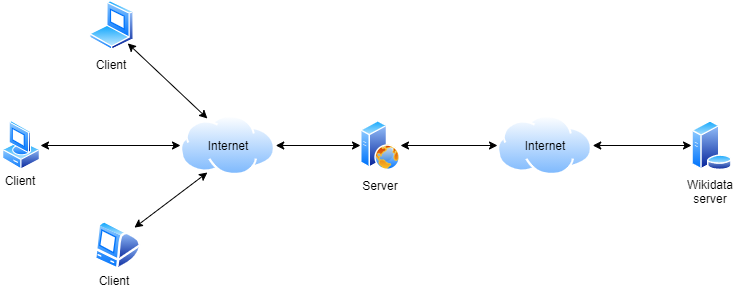
\includegraphics[width = 0.9\textwidth]{Imagenes/Bitmap/Diagrama cliente servidor.png}
	\caption{Diagrama de la arquitectura cliente-servidor de la aplicación}
	\label{fig:diagramaCS}
\end{figure}

Para explicar mejor su funcionamiento, estudiaremos cada una de las partes de la arquitectura por separado.\\

\subsection{Cliente}

El cliente es la parte con la que interactúan los usuarios de la aplicación. Como la nuestra es una aplicación web, el cliente es la parte del navegador y la interfaz visual que se muestra en el mismo.\\

En la interfaz se muestra la lista de canciones a elegir, la cual recibe desde el servidor mediante un archivo de formato CSV. Una vez el usuario escoja dos de esas canciones y confirme la selección, el cliente enviará una petición al servidor. El servidor realizará una serie de operaciones para comparar las canciones y obtener los grafos de explicaciones deseados.\\

Cuando el servidor haya completado su parte, devolverá al cliente un archivo de formato JavaScript donde están contenidas las estructuras de datos necesarias para dibujar los grafos. Empleando la librería vis.js, el cliente dibujará dos grafos y los mostrará por pantalla para que el usuario pueda verlos.\\

\subsection{Servidor}

El servidor es la parte que escucha las peticiones del cliente y hace las gestiones necesarias para devolverle la información deseada. Esta es la parte responsable de la mayoría de procesos existentes en nuestra aplicación, desde gestionar consultas a Wikidata hasta tratar los datos obtenidos para dibujar los grafos de explicaciones.\\

Para explicar el funcionamiento del servidor debemos repasar los módulos que lo conforman, cuya relación se puede observar en la Figura~\ref{fig:diagramaComponentes}.\\

\begin{figure}[h!]
	\centering
	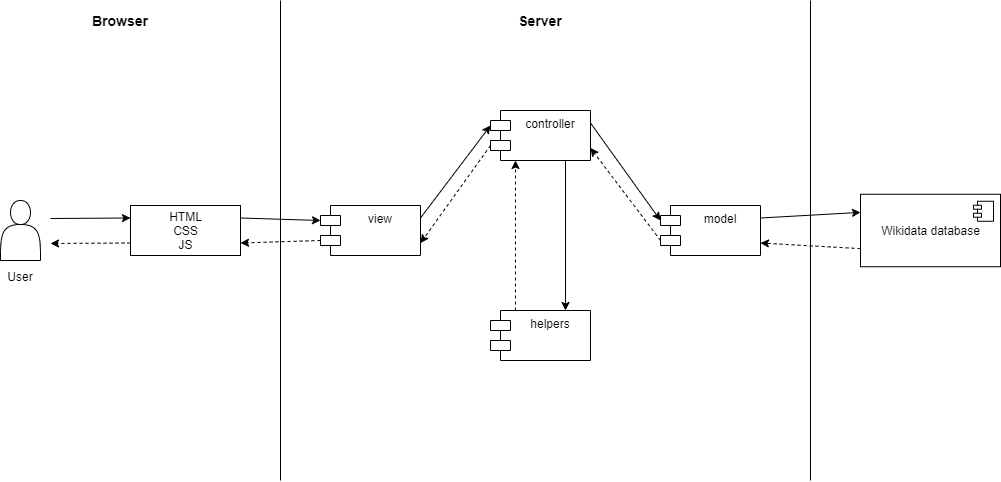
\includegraphics[width = 0.9\textwidth]{Imagenes/Bitmap/Diagrama componentes.png}
	\caption{Diagrama de componentes de la aplicación}
	\label{fig:diagramaComponentes}
\end{figure}

El módulo ``view'' contiene las plantillas de la interfaz, es decir, lo que verá el usuario por pantalla una vez se haya renderizado en el navegador.\\

El módulo ``controller'' es el centro de control entre el resto de módulos. Todas las comunicaciones entre módulos pasan por aquí. Recibe las peticiones de ``view'', que se originan por las elecciones del usuario, y a su vez pide al módulo ``model'' que gestione esa petición y devuelva los resultados. Con los resultados de ``model'', ``controller'' le pide al módulo ``helpers'' que procese esos datos para poder dibujar los grafos, tras lo cual ya está listo para devolver los resultados a ``view''.\\

El módulo ``model'' es uno de los más importantes. Se encarga de organizar los datos con los que se trabaja en la aplicación en clases, además de comunicarse con el servidor de Wikidata para obtener la información en la que se basan las explicaciones del sistema. Hace las consultas SPARQL y recoge los resultados en estructuras de datos con las que pueda trabajar el resto de la aplicación.\\

Por último, el módulo ``helpers'' es un módulo auxiliar para el dibujo de los grafos. Recibe los datos obtenidos de las consultas y los procesa para generar un archivo JavaScript que contiene las instrucciones necesarias para generar los grafos. Este será el que utilice el cliente para mostrar los grafos de explicaciones al usuario.\\

\subsection{Comunicación}

La comunicación con el servidor de Wikidata, se hace mediante el módulo ``model''. Este módulo se encarga de establecer la conexión con el punto de consultas de Wikidata para poder iniciar las consultas y recoger los datos devueltos. Como punto principal, encontramos la librería que nos ha permitido todas estas funciones SPARQLWrapper. La librería SPARQLWrapper permite el intercambio de información con la API de Wikidata, la cual está conectada a la base de datos. Permite búsquedas de menor a mayor complejidad aunque con un número de requests limitado. Nuestro modelo se va a encargar de obtener todas las propiedades requeridas sobre cada par canción-artista, clasificarla en función del nivel o categoría de cada una de ellas.\\


La conexión será establecida cada vez que el usuario quiera hacer una comparación entre un par de canciones, es decir el servidor hace una llamada por cada caso de uso que se quiera probar.\\

\begin{figure}[h!]
	\centering
	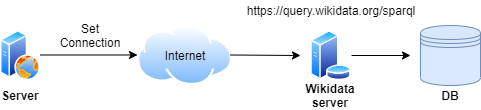
\includegraphics[width = 0.9\textwidth]{Imagenes/Bitmap/setConnection.png}
	\caption{Diagrama para establecer una conexión}
	\label{fig:diagramaConexion}
\end{figure}

\begin{figure}[h!]
	\centering
	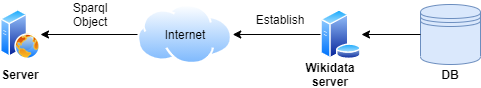
\includegraphics[width = 0.9\textwidth]{Imagenes/Bitmap/conexionReturn.png}
	\caption{Respuesta del servidor de Wikidata}
	\label{fig:respuestaWikidata}
\end{figure}

Una vez que obtengamos el objeto SPARQL que devuelve el servidor de Wikidata, ya podemos utilizarlo reiteradamente para poder mandar búsquedas al servidor de Wikidata. Estas búsquedas están definidas previamente, ya que todas las propiedades que serán objeto de estudio están recogidas en nuestro servidor y son las mismas para cada caso de uso. 
\\

\begin{figure}[h!]
	\centering
	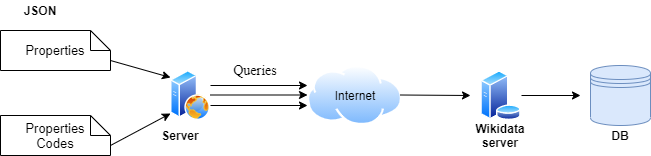
\includegraphics[width = 0.9\textwidth]{Imagenes/Bitmap/conexion.png}
	\caption{Lanzamiento de queries al servidor}
	\label{fig:queriesServidor}
\end{figure}

Como acabamos de explicar, la entrada común para todo caso de uso en nuestro modelo de la aplicación siempre es la misma: El par de canciones y el conjunto de propiedades que se va a estudiar sobre ellas para poder hallar las explicaciones. Las propiedades, junto con sus respectivos códigos de búsqueda, están guardados en formato JSON y CSV, los cuales al inicio del proceso serán reconvertidos en diccionarios para poderlos procesar con las clases del modelo. Todas consultas realizadas son devueltas en formato JSON, el cual es transformado a dataframe para poder operar más fácilmente con toda la información recogida.\\

Contamos con una jerarquía de clases, las cuales completan el módulo de conexión. Se encargarán de procesar las repuestas del servidor y crear progresivamente, a medida que nos llegan respuestas, varios documentos que contengan todas las propiedades de cada canción y las relacionen entre sí para poder obtener un grafo representable.\\

\section{Extensibilidad de la aplicación}

Se ha intentado dar un enfoque lo más aproximado posible a una estructura MVC~(Modelo-Vista-Controlador), con tal de poder hacer una aplicación lo reutilizable y atenta a posibles cambios o modificaciones. Con esto, hemos intentado que culaquier posible cambio referente al estudio sólo tuviese que modificar el modelo.\\

Poniendo un ejemplo, imaginemos que Wikidata implementa nuevas propiedades y códigos en la base de datos. Nuestras propiedades y sus respectivos códigos como hemos explicado anteriormente, están guardadas en ficheros JSON que al inicio de cada lanzamiento, son transformados en diccionarios. Contamos con métodos de adición los cuáles con tan solo obtener el nombre y el código de esa nueva propiedad y añadirlos a los ficheros JSON. El modelo no sufriría cambios en el código, ya que importa en cada lanzamiento todos estos diccionarios estáticos. De hecho, Wikidata es una base de datos que cambia constantemente por acción de diversos usuarios que completan y actualizan documentos constantemente, así que no es de extrañar que en cierto tiempo las explicaciones y por ende las propiedades activas, se queden obsoletas.\\\

En cuanto a la extensibilidad del DataSource de canciones y artistas, si necesitásemos añadir una nueva canción de un determinado artista, sería un caso distinto. Toda tupla canción-artista, debe sufrir un parseo y test previo a su adición al datasource. Esta, no es una función que se pueda lanzar desde el main de la aplicación porque no está pensada para añadir canciones a voluntad por motivos de compatibilidad con la sintaxis y el manejo que Wikidata hace sobre sus datos. Hay varios motivos como por ejemplo, el que la canción deseada no se encuentre en la base de datos de Wikidata o también que las letras iniciales de cada palabra estén guardadas en mayúsculas.\\

\section{Tecnologías y Herramientas utilizadas}
\label{sec:tecnologias}

Para la elaboración de este proyecto hemos tenido que estudiar numerosas tecnologías y herramientas diferentes. Algunas de ellas son viejas conocidas mientras que otras son completamente nuevas para nosotros y hemos tenido que familiarizarnos con ellas para poder trabajar con ellas.\\

A continuación haremos un repaso a las más relevantes para el desarrollo del proyecto, separándolas en distintos ámbitos para mayor comodidad.\\

\subsection{Programación}

\subsection*{Python}

Ha sido el lenguaje de programación principal, al menos en la parte del backend tanto para el núcleo del código que obtiene y relaciona los datos como para la creación de distintos scripts de ayuda, además de numerosas funciones para tratar los datos a representar en los grafos finales. Lo hemos escogido debido a su versatilidad y a su gran adaptación debido a la cantidad de librerías con las que cuenta.

\subsection*{Pandas y Numpy}

Dos librerías propias de Python, especializadas en el manejo y procesamiento de datos. Han sido de una utilidad vital ya que en gran parte del trabajo trabajamos con numerosos datasets y estas librerías nos proporcionan todo lo necesario para tratarlos, pudiendo así trabajar con ellos más fácilmente.

\subsection*{Sanic}

El framework seleccionado para desarrollar nuestra aplicación. Es un framework web asíncrono para Python cuyo objetivo es proporcionar una forma de crear un servidor que sea rápido y fácil de usar \cite{sanic}. Su sencillez para empezar a utilizarlo es uno de los principales factores que nos hizo decantarnos por él en lugar de otras opciones.

\subsection*{Jinja2}

Un motor de plantillas para Python basado en el sistema de plantillas de Django. Permite trabajar con documentos HTML con marcadores de posición que son llenados por lo que se le indica desde el código Python, permitiendo así utilizar variables en las vistas.\\

Esta función se utilizaba en una versión antigua de nuestro proyecto para tratar correctamente documentos cuyo título depende de la fecha y hora de su creación. Más adelante se cambió la forma en que se trataban estos documentos, pero seguimos utilizando Jinja2 para el formato de uso de las plantillas.

\subsection*{SPARQLWrapper}

Un wrapper para Python que permite ejecutar consultas SPARQL de forma remota \cite{sparqlwrapper}. Proporciona una funcionalidad esencial para nuestro trabajo, pues es lo que utilizamos para obtener la información de Wikidata desde nuestra aplicación.

\subsection*{HTML y CSS}

Dos lenguajes fundamentales para la programación web. Debido a la naturaleza de nuestra aplicación hemos recurrido a estos lenguajes para darle forma y estilo a la interfaz de explicaciones, aquella parte de nuestro proyecto con la que interactuarán los usuarios.

\subsection*{Javascript}

Al igual que los anteriores, este es un lenguaje de programación muy importante para el desarrollo web. Javascript es una parte integral de nuestro proyecto, pues es el lenguaje en el que se ha desarrollado la parte encargada de dibujar los grafos de explicaciones, además de otras funciones necesarias para el funcionamiento de la interfaz.

\subsection*{vis.js}

Esta es una librería de Javascript para visualización de datos  \cite{visjs}. Permite diversas representaciones gráficas, pero nosotros hemos empleado el componente Network para dibujar nuestros grafos de explicaciones. Es una librería bastante completa y con una documentación bien organizada, así que fue muy útil a la hora de plasmar en pantalla el resultado de nuestra investigación.

\subsection*{Jupyter-Notebooks}

Es un entorno informático interactivo basado en la web. Fue un entorno apropiado para realizar la prueba de scripts que nos ayudaron a limpiar y probar el dataset original.

\subsection{Organización}

\subsection*{Github}

Para poder almacenar y organizar todo el código en el que hemos trabajado conjuntamente. Nos ha permitido llevar un historial de versiones y actualizaciones de cada módulo del código. Github ha sido una herramienta apropiada no solo para llevar un control del código de la aplicación, sino también para la construcción de este mismo documento.

\subsection*{Google Drive}

Empleamos el servicio de alojamiento de archivos en la nube de Google para recoger y poner en común todos los documentos relacionados con la investigación previa al inicio del trabajo, además de para compartir recursos durante la realización del mismo. Su importancia quedó relegada a un segundo plano a medida que avanzaba el proyecto debido a que comenzamos a utilizar Github, pero cabe resaltar su utilidad durante las primeras fases.

\subsection*{Google Meet}

La aplicación de videoconferencias de Google fue una herramienta clave para mantener el contacto tanto con los directores del TFG como entre los miembros del equipo. Cuando las reuniones presenciales dejaron de ser posibles por motivos ajenos a nuestro control, se hizo necesario el uso de un servicio como este.

\subsection{Memoria}

\subsection*{LaTeX}

Este ha sido el procesador de textos elegido para la realización de este documento: la Memoria del TFG. Nos decantamos por este en lugar de otros procesadores como Word debido a las muchas posibilidades que tiene para generar documentos de calidad. Puntos como la estructura de capítulos, la estandarización de títulos o la forma de mostrar figuras (tanto imágenes como fragmentos de código), han hecho que nos resulte más sencilla la tarea de desarrollar esta memoria.

\subsection*{TeXiS}

TeXiS es una plantilla de \LaTeX para Tesis, Trabajos de Fin de Máster y otros documentos desarrollada por Marco Antonio y Pedro Pablo Gómez Martín. Es la plantilla que se ha usado como base para construir este documento y ha resultado de gran ayuda tanto para cuestiones de organización como para aprender a usar varias funcionalidades de \LaTeX, lo cual ha sido muy importante debido a nuestra falta de experiencia previa a este proyecto.

\subsection{Tecnologías y herramientas descartadas}

\subsection*{RDFstarTools}

Esta es una colección de librerías Java y herramientas de línea de comandos para procesar datos RDF* y consultas SPARQL* \cite{rdfstartools}. Proporciona varias funcionalidades, pero la verdaderamente relevante para nuestro proyecto es SPARQL* Parser, que sirve para hacer consultas SPARQL. Este parser está implementado sobre el framework Apache Jena.\\


Esta fue una de las opciones que barajamos para hacer consultas SPARQL desde nuestro código, pero acabamos decidiendo usar SPARQLWrapper en su lugar debido a que RDFstarTools es una colección de librerías de las cuales solo nos haría falta una pequeña parte. Tomando en consideración ambas opciones, nos pareció más adecuado utilizar Python junto con SPARQLWrapper debido ya que era más conciso y sencillo de implementar.

\subsection*{Java}

Uno de los lenguajes de programación de programación más extendidos y populares, especializado en la programación orientada a objetos. Al principio del proyecto nos planteamos utilizarlo como lenguaje principal para el backend de nuestra aplicación, sin embargo finalmente nos decantamos por Python.\\

Como ya hemos comentado antes, al decidir usar SPARQLWrapper para nuestras consultas SPARQL en lugar de RDFstarTools también nos pareció más adecuado descartar Java en favor de Python, aunque ambos habrían sido elecciones viables. 

\subsection*{Alchemy.js}

Alchemy.js es una aplicación de visualización de grafos para la web \cite{alchemyjs}. Está escrita en JavaScript con la librería D3.js como base y ofrece una manera sencilla y rápida de generar grafos. La mayoría de su personalización se lleva a cabo sobrescribiendo sus configuraciones por defecto, por lo que no requiere apenas implementar código JavaScript adicional.\\

Fue la primera opción contemplada para representar los grafos de nuestro proyecto debido a su sencillez de manejo y a su uso de archivos JSON para aportar los datos, algo que resultaba atractivo en un principio. Tras trabajar con ella durante un tiempo fue necesario descartarla por ciertas limitaciones a la hora de personalizar la representación según nuestro diseño, además de la falta de soporte por tratarse de un proyecto actualmente abandonado.

\chapter{Conclusiones y Trabajo Futuro}
\label{cap:conclusiones}

En este capítulo exponemos nuestras reflexiones respecto al trabajo realizado a lo largo del proyecto y los siguientes pasos a tomar en caso de continuarlo.\\

\section{Conclusiones}

Tras trabajar con la Web Semántica y Linked Data, hemos podido comprobar que son métodos de organización de datos con mucho potencial y del que todos podríamos beneficiarnos si se explora más allá de su estado actual. Su mayor inconveniente quizás sea precisamente que su utilidad depende en gran medida de lo extendido que esté su uso y, por desgracia, actualmente no está tan normalizado como nos gustaría.\\

Tomando como ejemplo el dominio en el que hemos centrado nuestro proyecto podemos ver estas limitaciones. Gracias a Linked Data y el formato RDF hemos sido capaces de obtener una buena cantidad de información que nos ha permitido generar explicaciones para la relación existente entre muchas canciones diferentes, sin embargo este trabajo no es suficiente para aplicar el mismo tratamiento a todas las obras musicales existentes, ni siquiera en la plataforma que hemos elegido para la obtención de datos.\\

Escogimos la web Wikidata para estudiar las canciones debido a su tamaño y a que utiliza efectivamente el modelo de datos enlazados. No obstante, esta plataforma dista mucho de ser perfecta debido a que no alberga la misma cantidad de información de todos sus elementos incluso aunque esa información exista, por lo que hay canciones que hemos podido explorar en más profundidad que otras. Por otra parte también hay casos de información poco fiable o directamente incorrecta, un problema con el que nos hemos topado en alguna ocasión y que provoca que no se pueda utilizar nuestra aplicación correctamente en esos casos.\\

A pesar de los problemas mencionados, Wikidata sigue siendo la mejor opción que hemos encontrado para alojamiento de información de música. Otras plataformas no hacen uso de Linked Data o lo hacen de tal forma que resulta muy difícil establecer relaciones en sus elementos porque son excesivamente concretos, llegando a tener muchas entradas diferentes para elementos que son iguales en esencia. Trabajos como el nuestro se beneficiarían de una mayor variedad en la oferta de bases de conocimiento que aprovechen las ventajas de la Web Semántica.\\

Centrándonos más en nuestro trabajo, consideramos que hemos logrado alcanzar la mayoría de nuestros objetivos propuestos. Gracias al estudio realizado de la Web Semántica y Linked Data, además de otras tecnologías, hemos alcanzado las conclusiones expuestas anteriormente. También hemos desarrollado un prototipo funcional de aplicación para mostrar el resultado de aplicar esas técnicas a las explicaciones de un recomendador. Todavía se podría continuar trabajando para mejorar y completar nuestro proyecto, pero estamos satisfechos con el resultado conseguido.\\

\section{Trabajo futuro}

Teniendo en cuenta que uno de nuestros objetivos es justificar de forma comprensible las recomendaciones de un sistema de recomendación, la evaluación con usuarios sería muy útil para determinar si se ha logrado alcanzar esta meta. No nos ha sido posible realizarla en esta versión del trabajo por falta de tiempo y complicaciones relacionadas con la situación extraordinaria de este año, pero sería el primer paso para mejorar nuestro proyecto.\\

El esquema RDF y el uso de SPARQL para su uso y análisis puede ser muy potente y abarcar grandes cantidades de datos. En nuestro caso nos hemos centrado en trabajar con la herramienta y los datos de Wikidata por una cuestión de cantidad de información, fiabilidad y resultados obtenidos. Con Wikidata hemos sido capaces de establecer conexiones entre canciones con toda la información posible en cada una de sus respectivas páginas descriptivas. Sin embargo hay más opciones de donde recopilar más información sobre canciones y artistas.\\ 

En un principio intentamos obtener información que se alejaba un poco más de lo que hemos creado, que es un análisis musical. Hay otras opciones y datos que se pueden sacar sobre canciones, como por ejemplo las películas o series en las que aparecen como banda sonora, o también canciones que han sido emitidas durante grandes eventos como la Superbowl. El problema que tuvimos es que el proyecto en ese punto se desviaba de su rumbo original, ya que en Wikidata no había datos tan específicos para la gran mayoría de canciones y debíamos recurrir a otras fuentes.\\

El problema de otras bases de datos alternativas es que tampoco poseen ese tipo de información tan detallada, no siguen el modelo de datos RDF o tienen la información tan solo en casos muy concretos y sin una forma efectiva de acceder a ella a partir de nuestro dataset, como comprobamos al estudiar la posibilidad de utilizar \textbf{MusicBrainz}~\cite{musicbrainz} para obtener las bandas sonoras en las que aparece una canción.\\

Otro aspecto en el que se puede trabajar para llegar a un trabajo mucho más completo y poder hacer una explicación de la relación de dos canciones, sería un estudio a nivel de usuario.
En nuestro proyecto hemos hecho un análisis avanzado de las relaciones que tienen las entidades en un ámbito musical. Sin embargo, hay otro estudio posible que es el análisis de los usuarios que han escuchado esas canciones. Partimos de la base de que dos personas que escuchan una misma canción, pueden compartir parte de sus gustos musicales, y se pueden recomendar y crear relaciones conforme a su historial.\\

Cada usuario tiene un historial de temas escuchados, de hecho uno de los datasets que obtuvimos al principio del proyecto era de este carácter. Si se hiciese un estudio individual de un usuario, se podrían analizar sus gustos musicales, canciones más escuchadas, últimos géneros más populares, etc.\\

Como ejemplo podemos seleccionar un usuario cuya mayoría de temas escuchados pertenecen al género pop, pero también cuenta con algunos pertenecientes al género indie durante los últimos meses. Si se encuentra una tendencia similar entre una cantidad significativa de usuarios, podríamos sacar una explicación que establezca una relación entre un tema de género pop y otro de género indie por la frecuencia con que aparecen estos géneros juntos entre las listas de temas escuchados de estos usuarios mencionados.\\


%%%%%%%%%%%%%%%%%%%%%%%%%%%%%%%%%%%%%%%%%%%%%%%%%%%%%%%%%%%%%%%%%%%%%%%%%%%
% Si el TFM se escribe en inglés, comentar las siguientes líneas 
% porque no es necesario incluir nuevamente las Conclusiones en inglés
\begin{otherlanguage}{english}
\chapter{Introduction}
\label{cap:introduction}

Since the development of the Internet as a global network, it has always hosted large amounts of documents and written information. As it grew, different ways had to be found to organize that information so that it could be used as a service to any user. The Semantic Web, whose characteristics we will explain later, is one of the methods that the entire Internet was able to adapt when it came to giving a meaning and a utility to that information.\\

The Semantic Web tries to link all that information in order to give it context and accessibility. To do this, it adopts the method of Linked Data, which, referring to its own name, connects or links different data establishing a relationship. The main objective of this is to give computers the ability to navigate and access most of the data stored on the Internet so that they are useful and not lost in a sea of information.\\

It is through this concept that search engines can be helped by this technology, as we provide machines the ability to navigate over those relationships and understand data that we require or could be useful to us.\\

In this project we will try to use Linked Data technology to enrich a music recommender system, providing explanations that justify its recommendations.\\

\section{Motivation}

The goal of this project is to give explanations to a music recommender. We start from a music recommender that provides a song to the user based on another song he has listened to, allegedly because there is some kind of relationship between them. Using that premise, we want to explain \textbf{why} those two songs are related or, in other words, how they resemble each other. To achieve this goal we will use the semantic web.\\

As we mentioned, the Semantic Web is a way to improve the connection between the data stored in the net, making the Internet more useful and accessible to people. The problem is that it is a practice that is not widespread enough to represent a real advance in our way of relating to the network yet, because it requires making changes in the way information is stored. In this paper we will try to show the potential of the Semantic Web.\\

The main point is to be able to collect all the connections that appear between all the information that we can get from each of the two musical themes or songs. For this, we must study that entity and all related: artist who performs the song, its musical genre, the members of its band, its record label, etc. and in turn the relations between them, until we have enough connections that can guarantee that those two songs have some relationship.\\

The connections obtained are explanations, which justify the relationship established by the system between two entities.\\

\section{Objectives}

The main objectives of this project are:

\begin{itemize}
\item To make a study on the Semantic Web and the data models that allow it, with the aim of developing later an application that exemplifies the practical applications that this Semantic Web can have.\\

\item To determine which properties may be most useful to establish explanations for the relationship between two provided songs, even if they are not very similar musically but share other interesting elements. This is the premise of our project and, thanks to our research, we will be able to determine which properties are most important when obtaining meaningful explanations in the domain.\\

\item To study different technologies that help us in the elaboration of the aforementioned application, in addition to expanding our knowledge in areas of computer science that we have not necessarily explored during the degree.\\

\item To design a visual interface of explanations, using iterative development that allows us to obtain a satisfactory result. This development includes the implementation of the design in our application.\\

\item Once completed, draw conclusions about the work done and set tasks to be performed in a future development.\\
\end{itemize}

\section{Work plan}

After explaining the motivation of this project and the objectives proposed for it, we proceed to detail the stages crossed in the development process.\\

Initially we became familiar with the Semantic Web and Linked Data, as well as some of the related technologies. This research has been detailed in Chapter~\ref{cap:estadoDeLaCuestion}.\\

Then we established the list of explanations that we would use in the final version of the application, which is collected and explained in Chapter~\ref{cap:explicaciones}.\\

Later we started the development of the application, starting with the design of the explanation interface (documented in Chapter~\ref{cap:interfaz}) and continuing with the implementation, including its architecture and functionality. This process is explained in the Chapter~\ref{cap:implementacion}.\\

Finally, we reflected on the work done and the subject studied throughout the project. These conclusions are noted in Chapter~\ref{cap:conclusions}, as well as the future work we should do if we continued to develop the application.\\
\chapter{Conclusions and Future Work}
\label{cap:conclusions}

Conclusions and future lines of work. This chapter contains the translation of Chapter \ref{cap:conclusiones}.



\end{otherlanguage}
%%%%%%%%%%%%%%%%%%%%%%%%%%%%%%%%%%%%%%%%%%%%%%%%%%%%%%%%%%%%%%%%%%%%%%%%%%%

%
% Bibliografía
%
% Si el TFM se escribe en inglés, editar TeXiS/TeXiS_bib para cambiar el
% estilo de las referencias
%---------------------------------------------------------------------
%
%                      configBibliografia.tex
%
%---------------------------------------------------------------------
%
% bibliografia.tex
% Copyright 2009 Marco Antonio Gomez-Martin, Pedro Pablo Gomez-Martin
%
% This file belongs to the TeXiS manual, a LaTeX template for writting
% Thesis and other documents. The complete last TeXiS package can
% be obtained from http://gaia.fdi.ucm.es/projects/texis/
%
% Although the TeXiS template itself is distributed under the 
% conditions of the LaTeX Project Public License
% (http://www.latex-project.org/lppl.txt), the manual content
% uses the CC-BY-SA license that stays that you are free:
%
%    - to share & to copy, distribute and transmit the work
%    - to remix and to adapt the work
%
% under the following conditions:
%
%    - Attribution: you must attribute the work in the manner
%      specified by the author or licensor (but not in any way that
%      suggests that they endorse you or your use of the work).
%    - Share Alike: if you alter, transform, or build upon this
%      work, you may distribute the resulting work only under the
%      same, similar or a compatible license.
%
% The complete license is available in
% http://creativecommons.org/licenses/by-sa/3.0/legalcode
%
%---------------------------------------------------------------------
%
% Fichero  que  configura  los  parámetros  de  la  generación  de  la
% bibliografía.  Existen dos  parámetros configurables:  los ficheros
% .bib que se utilizan y la frase célebre que aparece justo antes de la
% primera referencia.
%
%---------------------------------------------------------------------


%%%%%%%%%%%%%%%%%%%%%%%%%%%%%%%%%%%%%%%%%%%%%%%%%%%%%%%%%%%%%%%%%%%%%%
% Definición de los ficheros .bib utilizados:
% \setBibFiles{<lista ficheros sin extension, separados por comas>}
% Nota:
% Es IMPORTANTE que los ficheros estén en la misma línea que
% el comando \setBibFiles. Si se desea utilizar varias líneas,
% terminarlas con una apertura de comentario.
%%%%%%%%%%%%%%%%%%%%%%%%%%%%%%%%%%%%%%%%%%%%%%%%%%%%%%%%%%%%%%%%%%%%%%
\setBibFiles{%
bibliography
}

%%%%%%%%%%%%%%%%%%%%%%%%%%%%%%%%%%%%%%%%%%%%%%%%%%%%%%%%%%%%%%%%%%%%%%
% Definición de la frase célebre para el capítulo de la
% bibliografía. Dentro normalmente se querrá hacer uso del entorno
% \begin{FraseCelebre}, que contendrá a su vez otros dos entornos,
% un \begin{Frase} y un \begin{Fuente}.
%
% Nota:
% Si no se quiere cita, se puede eliminar su definición (en la
% macro setCitaBibliografia{} ).
%%%%%%%%%%%%%%%%%%%%%%%%%%%%%%%%%%%%%%%%%%%%%%%%%%%%%%%%%%%%%%%%%%%%%%
\setCitaBibliografia{
\begin{FraseCelebre}
\begin{Frase}
  Y así, del mucho leer y del poco dormir, se le secó el celebro de
  manera que vino a perder el juicio.\\ 
  \textcolor{red}{(modificar en Cascaras$\backslash$bibliografia.tex)}
\end{Frase}
\begin{Fuente}
  Miguel de Cervantes Saavedra
\end{Fuente}
\end{FraseCelebre}
}

%%
%% Creamos la bibliografia
%%
\makeBib

% Variable local para emacs, para  que encuentre el fichero maestro de
% compilación y funcionen mejor algunas teclas rápidas de AucTeX

%%%
%%% Local Variables:
%%% mode: latex
%%% TeX-master: "../Tesis.tex"
%%% End:



% Apéndices
\appendix
\chapter{Título del Apéndice A}
\label{Appendix:Key1}

Contenido del apéndice
%\chapter{Título del Apéndice B}
\label{Appendix:Key2}

%\include{Apendices/appendixC}
%\include{...}
%\include{...}
%\include{...}
\backmatter



%
% Índice de palabras
%

% Sólo  la   generamos  si  está   declarada  \generaindice.  Consulta
% TeXiS.sty para más información.

% En realidad, el soporte para la generación de índices de palabras
% en TeXiS no está documentada en el manual, porque no ha sido usada
% "en producción". Por tanto, el fichero que genera el índice
% *no* se incluye aquí (está comentado). Consulta la documentación
% en TeXiS_pream.tex para más información.
\ifx\generaindice\undefined
\else
%%---------------------------------------------------------------------
%
%                        TeXiS_indice.tex
%
%---------------------------------------------------------------------
%
% TeXiS_indice.tex
% Copyright 2009 Marco Antonio Gomez-Martin, Pedro Pablo Gomez-Martin
%
% This file belongs to TeXiS, a LaTeX template for writting
% Thesis and other documents. The complete last TeXiS package can
% be obtained from http://gaia.fdi.ucm.es/projects/texis/
%
% This work may be distributed and/or modified under the
% conditions of the LaTeX Project Public License, either version 1.3
% of this license or (at your option) any later version.
% The latest version of this license is in
%   http://www.latex-project.org/lppl.txt
% and version 1.3 or later is part of all distributions of LaTeX
% version 2005/12/01 or later.
%
% This work has the LPPL maintenance status `maintained'.
% 
% The Current Maintainers of this work are Marco Antonio Gomez-Martin
% and Pedro Pablo Gomez-Martin
%
%---------------------------------------------------------------------
%
% Contiene  los  comandos  para  generar  el índice  de  palabras  del
% documento.
%
%---------------------------------------------------------------------
%
% NOTA IMPORTANTE: el  soporte en TeXiS para el  índice de palabras es
% embrionario, y  de hecho  ni siquiera se  describe en el  manual. Se
% proporciona  una infraestructura  básica (sin  terminar)  para ello,
% pero  no ha  sido usada  "en producción".  De hecho,  a pesar  de la
% existencia de  este fichero, *no* se incluye  en Tesis.tex. Consulta
% la documentación en TeXiS_pream.tex para más información.
%
%---------------------------------------------------------------------


% Si se  va a generar  la tabla de  contenidos (el índice  habitual) y
% también vamos a  generar el índice de palabras  (ambas decisiones se
% toman en  función de  la definición  o no de  un par  de constantes,
% puedes consultar modo.tex para más información), entonces metemos en
% la tabla de contenidos una  entrada para marcar la página donde está
% el índice de palabras.

\ifx\generatoc\undefined
\else
   \addcontentsline{toc}{chapter}{\indexname}
\fi


% Generamos el índice
\printindex

% Variable local para emacs, para  que encuentre el fichero maestro de
% compilación y funcionen mejor algunas teclas rápidas de AucTeX

%%%
%%% Local Variables:
%%% mode: latex
%%% TeX-master: "./tesis.tex"
%%% End:

\fi

%
% Lista de acrónimos
%

% Sólo  lo  generamos  si  está declarada  \generaacronimos.  Consulta
% TeXiS.sty para más información.


\ifx\generaacronimos\undefined
\else
%---------------------------------------------------------------------
%
%                        TeXiS_acron.tex
%
%---------------------------------------------------------------------
%
% TeXiS_acron.tex
% Copyright 2009 Marco Antonio Gomez-Martin, Pedro Pablo Gomez-Martin
%
% This file belongs to TeXiS, a LaTeX template for writting
% Thesis and other documents. The complete last TeXiS package can
% be obtained from http://gaia.fdi.ucm.es/projects/texis/
%
% This work may be distributed and/or modified under the
% conditions of the LaTeX Project Public License, either version 1.3
% of this license or (at your option) any later version.
% The latest version of this license is in
%   http://www.latex-project.org/lppl.txt
% and version 1.3 or later is part of all distributions of LaTeX
% version 2005/12/01 or later.
%
% This work has the LPPL maintenance status `maintained'.
% 
% The Current Maintainers of this work are Marco Antonio Gomez-Martin
% and Pedro Pablo Gomez-Martin
%
%---------------------------------------------------------------------
%
% Contiene  los  comandos  para  generar  el listado de acrónimos
% documento.
%
%---------------------------------------------------------------------
%
% NOTA IMPORTANTE:  para que la  generación de acrónimos  funcione, al
% menos  debe  existir  un  acrónimo   en  el  documento.  Si  no,  la
% compilación  del   fichero  LaTeX  falla  con   un  error  "extraño"
% (indicando  que  quizá  falte  un \item).   Consulta  el  comentario
% referente al paquete glosstex en TeXiS_pream.tex.
%
%---------------------------------------------------------------------


% Redefinimos a español  el título de la lista  de acrónimos (Babel no
% lo hace por nosotros esta vez)

\def\listacronymname{Lista de acrónimos}

% Para el glosario:
% \def\glosarryname{Glosario}

% Si se  va a generar  la tabla de  contenidos (el índice  habitual) y
% también vamos a  generar la lista de acrónimos  (ambas decisiones se
% toman en  función de  la definición  o no de  un par  de constantes,
% puedes consultar config.tex  para más información), entonces metemos
% en la  tabla de contenidos una  entrada para marcar  la página donde
% está el índice de palabras.

\ifx\generatoc\undefined
\else
   \addcontentsline{toc}{chapter}{\listacronymname}
\fi


% Generamos la lista de acrónimos (en realidad el índice asociado a la
% lista "acr" de GlossTeX)

\printglosstex(acr)

% Variable local para emacs, para  que encuentre el fichero maestro de
% compilación y funcionen mejor algunas teclas rápidas de AucTeX

%%%
%%% Local Variables:
%%% mode: latex
%%% TeX-master: "../Tesis.tex"
%%% End:

\fi

%
% Final
%
%%---------------------------------------------------------------------
%
%                      fin.tex
%
%---------------------------------------------------------------------
%
% fin.tex
% Copyright 2009 Marco Antonio Gomez-Martin, Pedro Pablo Gomez-Martin
%
% This file belongs to the TeXiS manual, a LaTeX template for writting
% Thesis and other documents. The complete last TeXiS package can
% be obtained from http://gaia.fdi.ucm.es/projects/texis/
%
% Although the TeXiS template itself is distributed under the 
% conditions of the LaTeX Project Public License
% (http://www.latex-project.org/lppl.txt), the manual content
% uses the CC-BY-SA license that stays that you are free:
%
%    - to share & to copy, distribute and transmit the work
%    - to remix and to adapt the work
%
% under the following conditions:
%
%    - Attribution: you must attribute the work in the manner
%      specified by the author or licensor (but not in any way that
%      suggests that they endorse you or your use of the work).
%    - Share Alike: if you alter, transform, or build upon this
%      work, you may distribute the resulting work only under the
%      same, similar or a compatible license.
%
% The complete license is available in
% http://creativecommons.org/licenses/by-sa/3.0/legalcode
%
%---------------------------------------------------------------------
%
% Contiene la última página
%
%---------------------------------------------------------------------


% Ponemos el marcador en el PDF
\ifpdf
   \pdfbookmark{Fin}{fin}
\fi

\thispagestyle{empty}\mbox{}

Este texto se puede encontrar en el fichero Cascaras/fin.tex. Si deseas eliminarlo, basta con comentar la línea correspondiente al final del fichero TFMTeXiS.tex.

\vspace*{4cm}

\small

\hfill \emph{--¿Qué te parece desto, Sancho? -- Dijo Don Quijote --}

\hfill \emph{Bien podrán los encantadores quitarme la ventura,}

\hfill \emph{pero el esfuerzo y el ánimo, será imposible.}

\hfill 

\hfill \emph{Segunda parte del Ingenioso Caballero} 

\hfill \emph{Don Quijote de la Mancha}

\hfill \emph{Miguel de Cervantes}

\vfill%space*{4cm}

\hfill \emph{--Buena está -- dijo Sancho --; fírmela vuestra merced.}

\hfill \emph{--No es menester firmarla -- dijo Don Quijote--,}

\hfill \emph{sino solamente poner mi rúbrica.}

\hfill 

\hfill \emph{Primera parte del Ingenioso Caballero} 

\hfill \emph{Don Quijote de la Mancha}

\hfill \emph{Miguel de Cervantes}


\newpage
\thispagestyle{empty}\mbox{}

\newpage

% Variable local para emacs, para  que encuentre el fichero maestro de
% compilación y funcionen mejor algunas teclas rápidas de AucTeX

%%%
%%% Local Variables:
%%% mode: latex
%%% TeX-master: "../Tesis.tex"
%%% End:

%\end{otherlanguage}
\end{document}
